\chapter{Theoretical Framework}\label{ch2:TheoFrame}

\section{Hydrogels}

%\paragraph{Introduction} 

From bibliographic review, we can say that a hydrogel is a polymeric network that has the capacity of swelling\citep{choiSynthesisHydrogelBasedMicrogels2025,dayTunableNetworkArchitecture2025,ahmedHydrogelPreparationCharacterization2015a,bustamante-torresHydrogelsClassificationAccording2021}.
Some examples are,
    polyacrylamide,
    sodium polyacrylate,
    Poly(vinyl alcohol),
    Poly(ethylene glycol),
    Poly(hydroxyyethyl methacrylate),
    agarose,
    alginate,
    gelatin,
    pectin,
    starch,
    cellulose-based networks,
    protein networks,
    among others.
In order to try to understand (some of) the properties of the hydrogels, we are going to explore what is a polymeric network and what is the capacity of swelling.

In general terms, a polymeric network is a three dimensional structure formed by long polymer chains that are interconnected.
Meanwhile, the swellability is defined as the capacity to absorb significant amounts of a solvent without dissolving, resulting in an increase volume.
Since the swellability is a ``capacity'' of the network, we are going to start by exploring what is a polymeric structure\citep{bustamante-torresHydrogelsClassificationAccording2021}.

\subsection{Polymeric networks}

%\paragraph{Introduction} 
From a structural perspective, polymer networks consist of network ``junctions'', which contain three or more strands connected by a mechanism. 
This mechanism is commonly refer as ``crosslink'' and can be describe through physical interactions or covalent bonds.
In contrast, it is important to note that a polymer is a macromolecule composed of monomers that are covalently bonded together to form a strand.
Monomers can possess specific functional groups or reactive sites, which determine the manner in which monomers bind together. 
This, in turn, influences the structural and property characteristics of the resulting polymer.
The swelling capacity can be attributed, at least in part, to the type of monomers in the network. 
The structural frameworks provide a comprehensive explanation of the mechanical response and the swelling.

%\paragraph{Swellability} 
The capacity for substantial solvent absorption and expansion of hydrogels is attributable to the expansion of the network due to osmotic pressure and the hydrophilic funcional groups of the monomers that constitute hydrogels.
Some of the key hydrophilic groups are,
    hydroxyl group,
    amide group,
    carboxylate anion,
    ether group.
The hydrophilic phenomenon, from a chemical perspective, occurs when molecules possess polar or charged functional groups that spontaneously form hydrogen bonds or electrostatic interactions with water, enabling water to diffuse over the surface.
Nevertheless, the network's integrity remains intact due to the crosslink mechanism\citep{lelePredictionsBoundWater1997}.

%\paragraph{Crosslink} 
The underlying principles of crosslink mechanism are the physical interactions and covalent bonds.
However it is important to acknolwdge that, for example, given sufficiently strong and static physical interactions, physical networks can behave identically to covalent bonded networks; 
alternatively, the incorporation of mechanisms for covalent bond exchange can result in chemical networks that exhibit adaptable mechanical properties regulated by external stimuli [cite]. 
Consequently, an emphasis on bond strengths and exchange rates provides more informative insights for accurately inferring the properties of hydrogels\citep{priyaComprehensiveReviewHydrogel2024}.

With this understanding, a covalent bond is defined as a specific type of chemical bond that occurs when two atoms share one or more pairs of electrons. 
On the other hand, a physical interaction is defined as a non-covalent force that describes how atoms, ions, or molecules attract or repel each other without forming new chemical entities. 
The covalent bond is the result of quantum mechanical interactions between atomic orbitals.
In these interactions, shared electrons occupy a molecular orbital that extends over both atoms. 
In contrast, physical interactions are attributed to electrostatic, van der Waals, or dipole forces, arising from the redistribution of electron density and the consequent energy alterations between particles.

Now we can dive into the different types of polymer networks and the different types of crosslink mechanisms.
After that, then we are going to spend some paragraphs into explore the ideas of mechanical response through constitutive relations.
In order to end with the mechanical response of hydrogels and some conections with the polymeric network.

\subsection{Types of polymeric networks: Gels}

%\paragraph{Introduction} 
In general terms a polymeric network can be divided into one of four major classes: 
    thermosets,
    thermoplastics,
    elastomers,
    and gels.
Thermosets are rigid, covalently bonded polymer networks with high modulus, which are insoluble and degrade rather than melt upon heating. 
In contrast, thermoplastics are held together by strong physical interactions, allowing them to be remolded and recycled when heated. 
Elastomers are soft, deformable with covalent networks used above their glass transition temperature, capable of large reversible extensions. 
Finally, gels are liquid-swollen networks, either covalent or physical interactions, that are soft and highly deformable.

%\paragraph{Gels} 
In detail, a gel is a three-dimensional, crosslinked polymer network formed by physical or chemical crosslinks, which serve to trap the solvent molecules via intermolecular interactions, including hydrogen bonding and osmotic forces. This process prevents the fluid from flowing freely.
This results in a material with both solid and liquid characteristics—elasticity from the polymer network and fluidity from the entrapped solvent.
This description resembles that of a hydrogel.
The hydrogel, however, is a specific type of gel in which the solvent is water and the polymers are hydrophilic.

%\paragraph{Gel point} 
The classification of a polymer network as a gel is characterized by the formation of a continuous, system-spanning (infinite) network through the process of polymerization or crosslinking mechanisms.
This phenomenon is indicative of the percolation\footnote{In physics, percolation describes the emergence of large-scale connectivity in disordered systems. On the other hand, mathematically, is the study of cluster formation in a random graph or lattice when sites or bonds are occupied with a given probability.} of the polymeric network.
And it is known as the gel point\citep{guPolymerNetworksPlastics2020}.
At this point, the polymer chains become sufficiently interconnected through crosslinks to create a macroscopic network that spans the entire volume, causing the material to gain elasticity and lose fluidity, transitionning\footnote{This transition is a percolation threshold where the molecular weight and network correlation length diverge.} it from a viscous liquid (sol) to a solid-like gel.

Finally, it must be mentioned that not all polymer networks can achieve a gel point.
To reach this point requires sufficient network connectivity due to enough reactive sites and a high enough crosslinking density.
For instance, linear, unbranched, or insufficiently crosslinked polymers remain soluble and do not gel.

\subsection{Crosslink mechanisms}

%\paragraph{Intro} 
According to the literature, the most common classification is typically as physical or covalent hydrogels.
In regards to the main crosslink mechanism present in the polymeric network.
However, it is important to note that, although the crosslink mechanism plays a significant role in network integrity, it is not the sole mechanism that can adequately describe the mechanical response in terms of network structure.
In this regard, three primary crosslink mechanisms can be identified: covalent, physical interactions, and mechanical\citep{bustamantetorresHydrogelsClassificationAccording2021}.

%\paragraph{Covalent Crosslinking} 
Polymer chains are linked by covalent bonds, which are typically formed through free-radical polymerization, click chemistry, or UV-induced reactions.
This results in a static, stable, and robust network with high mechanical strength and low reversibility.
However, when dynamic covalent chemistry is applied, it can allow bond exchange and self-healing properties.

%\paragraph{Physical Crosslinking} 
Polymer chains are held together by non-covalent interactions, including hydrogen bonding, ionic interactions, hydrophobic associations, and van der Waals forces.
Given the possibility of bond exchange under normal conditions, the network is dynamic.
Therefore, they tend to be softer and less mechanically robust in comparison to covalently crosslinked hydrogels.
Finally, these networks are reversible, enabling self-healing, shape-memory, and stimuli-responsive behaviors.

%\paragraph{Mechanical Crosslinking} 
Finally, these types of crosslinked networks are held together by physical entanglements or interpenetrating polymer chains.
Examples include double-network hydrogels, slide-ring gels, and highly entangled architectures.
This provides toughness and elasticity properties by dissipating energy through chain movement and entanglement.

\begin{figure}[!ht]
    \centering
    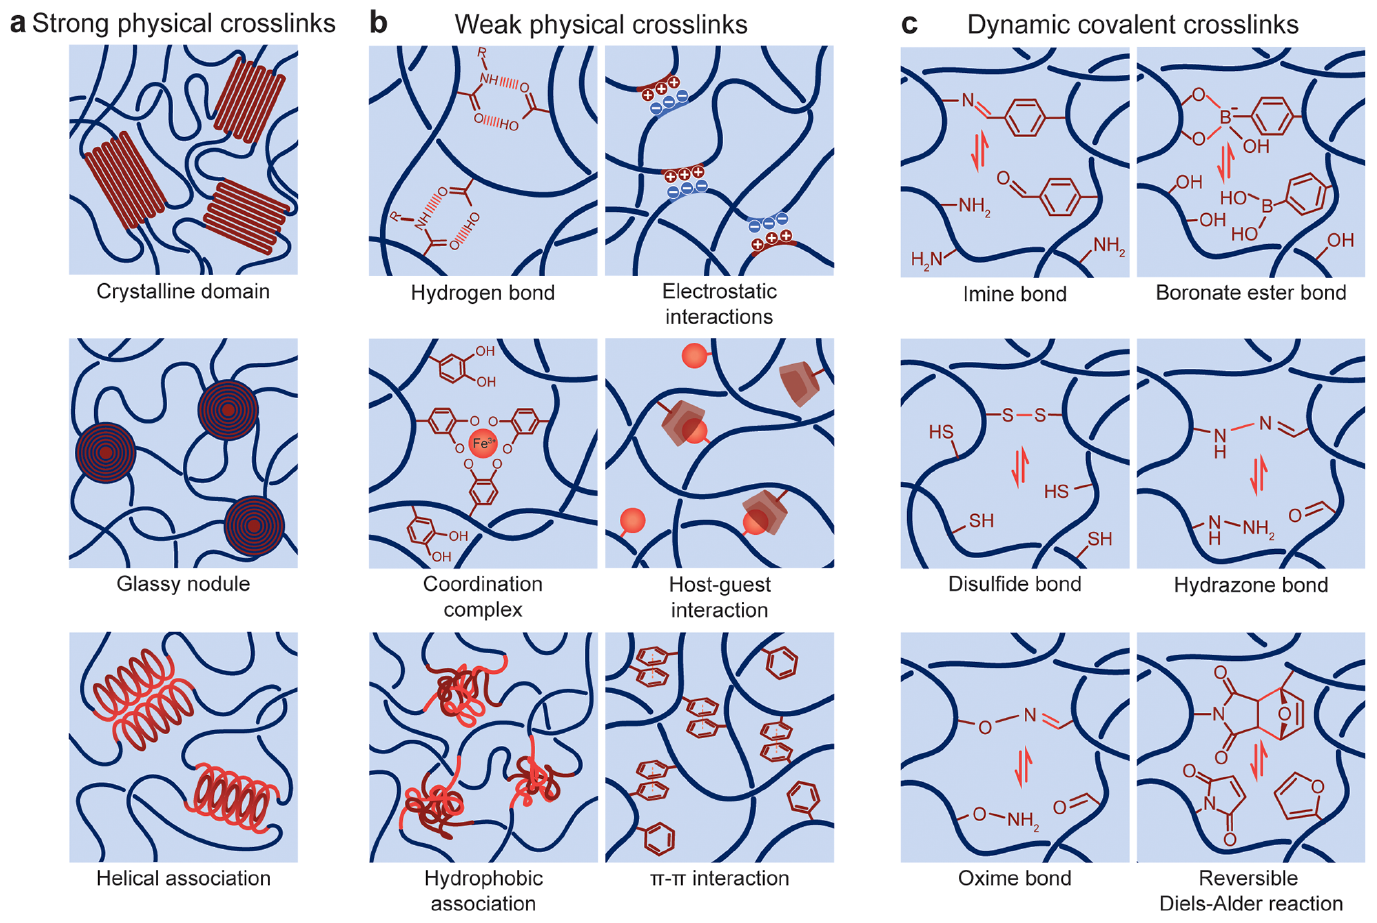
\includegraphics[width=0.8\textwidth]{figs/crosslinker_mechanisms.png}
    \caption{Image with the three different crosslinker mechanisms}
\end{figure}

\subsection{Reverible networks}

%\paragraph{Intro} 
Another common classification in literature is to categorize the polymeric network as reversible or irreversible.
It is a common association that networks with physical crosslink mechanisms are reversible, while covalently crosslinked networks are irreversible.
However, regardless of the crosslink mechanism, the network can be shown to be reversible.

%\paragraph{Physical networks} 
The interactions can spontaneously break and reform due to thermal fluctuations or changes in the microenviroment, sucha pH, ionic strength, temperature.
When external stress or energy disturbs the network, some physical bonds dissociate. 
Free chain segments then seek new partners, allowing dynamic rejoining at different sites. 
This ongoing exchange can lead to self-healing, viscoelastic behavior, and adaptability of the hydrogel.
The equilibrium and kinetics of bond formation/dissociation can be tuned by controlling the physical interactions.

%\paragraph{Covalent networks} 
In ``dynamic'' covalent bonds, such as imine, boronate ester, thioester, disulfide, and transesterification, the network has the capacity to break and reform via chemical equilibrium. 
This process is driven by external stimuli, including temperature, pH, or catalysts.
The external stimuli facilitate the exchange of polymer chains at crosslinked points through either associative or dissociative mechanisms.
The associative mechanism occurs when new bonds form before old bonds break. In contrast, the dissociative mechanism occurs when old bonds break before new bonds form.
The exchange of polymer chains enables the material to exhibit self-healing, stress relaxation, and shape adaptability while maintaining the mechanical strength provided by covalent bonds to the network.
Finally, it is important to note that the energy barrier for exchange, bond stability, and stimulus-dependence govern the rate and reversibility of the process.


\section{Mechanical response}

The concept of a material's mechanical response describes the relationship between the deformation of a material and the applied stress and/or shear rate.
Nevertheless, this relationship can be described from a macroscopic scale and also from a microscopic scale.
At the macroscopic level, the description captures the effective mechanical response as a continuum property. 
At the microscopic level, it provides insights into the origin of the mechanical response and how structural features at small scales control the macroscopic response.
In this section, we will delve into the various descriptions and explore the quantification of this relationship.

%\paragraph{Constitutive relations} 
The relationship between deformation and stress is expressed through a constitutive equation.
This equation is a mathematical tool that quantifies the relationship. 
It is used to predict or model material behavior, as reflected by empirical observations.
Additionally, these equations can be defined from both the microscopic and microscopic scale.
These two scales are linked through the implementation of averaging or homogenization procedures.
However, there is a difference in interpretation and application.
Thse issues will be addressed in the following sections.

%\paragraph{Tensors} 
Before proceeding, it is necessary to know the quantitative representation of stress and strain.
Both quantities are mathematically represented as second-rank tensors, which can be algebraically expressed as a $n\times n$ matrix.
Furthermore, it is important to interpret tensors as a generalization of scalars, vectors, and matrices to describe physical quantities which depend on direction and coordinate system, yet follow specific transformation rules under changes of coordinates.
Allowing to quantify not just the magnitud but also aorientation and how the physical quantity acts along different directions in space.
In summary, the tensor enables the capture of multidirectional physical properties that remain constant under coordinate changes.
Keeping this in mind, we can proceed with a description of the strain tensor. The stress tensor will be defined until the microscopic section, together with the relation to the microscopic-macroscopic relation.
This is due to the scope of the thesis.

%\paragraph{Strain} 
In physics, the deformation of a material relative to its original shape under applied forces is quantify by the relative displacement between points in the material.
This measure is represented by the dimensionless strain tensor,
\begin{gather}
    \epsilon_{ij} = \frac{1}{2}\left( \pdv{u_i}{x_j}+\pdv{u_j}{x_i} \right).\label{eqn:strainTensor}
\end{gather}
Where $u_i$ are the component of the displacement vector field and $x_j$ are the spatial coordinates.
This mathematical representation is only valid for infinitesimal small deformations and enables the description of normal strain, such as elongation or compression, through the use of diagonal terms, and shear strain via off-diagonal terms.
On figure~\ref{fig:strainTensor} is a visual representation of equation~\eqref{eqn:strainTensor} in a two spatial dimensional situation.
It is important to keep in mind that the strain tensor is the spatial derivative of the displacement, it does not take into account the distance or the path taken.

\begin{figure}[ht!]
    \centering
    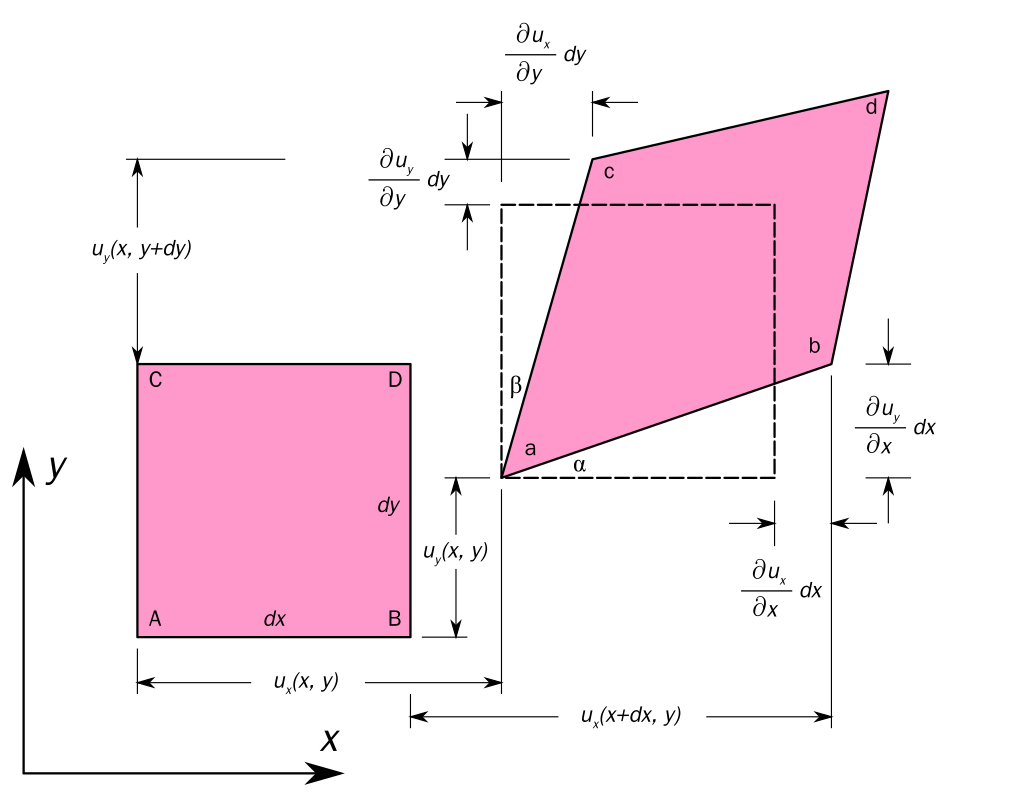
\includegraphics[width=0.8\textwidth]{figs/2D_geometric_strain.png}
    \caption{Strain representation Wikipedia}\label{fig:strainTensor}
\end{figure}

\subsection{Macroscopic description}

Now that we know how the quantify strain, we can quantify the four main mechanical responses,
    elastic,
    plastic,
    viscoelastic,
    and viscoplastic.
In a broad sense, the elastic relation is when the material returns to its original shape after load removal.
In contrast, the plastic deformation is a permanent deformation once stress exceeds a yield threshold $\sigma_y$.
Furthermore, the viscoelastic response is time-dependent combining the elastic and viscous behaviour.
Finally, the viscoplastic, combines the irriversible plastic strain with a rate-dependent viscous effects.

%\paragraph{Elastic relation} 
An elastic deformation is when the material returns to its original configuration once the stress is removed.
The quantification of this response is given by a linear equation,
\begin{gather}
    \sigma_{ij} = C_{ijkl}\epsilon_{kl}\label{eqn:elasticEQN}
\end{gather}
with a proportionality constant ($C_{ijkl}$) known as elastic modulus or Young's modulus.
The equation~\eqref{eqn:elasticEQN} is interpreted as the stiffness, that is how the material resists deformation.
Some examples of this type of deformation are the streching of a metal spring within its elastic limit or the compression of a rubber ball.

%This establishes a connection between the stress tensor ($\sigma$), the shear modulus ($G$) of the material, the applied strain ($E$), and the Lame first parameter ($\lambda$) of the material\citep{bonyadiReviewFrictionLubrication2020}.

%\paragraph{Plastic relation} 
In contrast, a plastic deformation is when the material has an irreversible change in the shape or size.
It is generally accepted that a material first enters an elastic regime and then reaches a yield point. 
After this point, the deformation is irreversible.
The quantification of the plastic relation typically links stress and plastic strain as a function of the current stress and internal variables,
\begin{gather}
    \dot{\bm{\epsilon}}_{p} = f\left(\bm{\sigma},\mathrm{Internal~varaibles}\right),\quad\bm{\sigma}>\bm{\sigma}_{y}\label{eqn:plasticEQN}.
\end{gather}
This is valid when the deformation goes beyond the yield stress and the specific algebraic expression is dictated by the material's properties.
The specific algebraic expression of $f\left(\bm{\sigma},\mathrm{Internal~varaibles}\right)$ depends on the material and conditions in which the deformation took place.

Furthermore, it is important to acknowledge that the definition of yield stress is also dependent on the material and the loading conditions\citep{bonnYieldStressMaterials2017}.
For this reason, there are many yield criteria developed for different materials and conditions, such as Drucker-Prager, Mohr-Coulomb, Von Mises or Tresca criterion.
The two most common yield criteria are the Von Mises and Tresca criterion.
The von Mises yield criterion it is commonly used for ductile materials.
It is base on the energy associated with shape change. 
This is defined by a critical value in terms of the distortional energy or equivalent shear stress and independent of hydrostatic pressure, 
\begin{gather}
    \sigma_y = \sqrt{\frac{3}{2}\bm{s}:\bm{s}}\label{eqn:vonMisesCriterion}
\end{gather}
where $\bm{s}$ is the deviatoric stress tensor\footnote{The stress tensor without the diagonal elements.} and $:$ is a tensor constraction, which maps a tensor to a scalar.
On the other hand, the Tresca yield criterion is a max-shear based criterion.
It is based on the yield strength in simple tension as follows, 
\begin{gather}
   \sigma_y = \max\left(\abs{\sigma_1-\sigma_2},\abs{\sigma_2-\sigma_3},\abs{\sigma_3-\sigma_1}\right)\label{eqn:trescaCriterion}
\end{gather}
where $\sigma_1=\sigma_{11}$, $\sigma_2=\sigma_{22}$, $\sigma_3=\sigma_{33}$ are also known as the principal stresses.

%\paragraph{Viscoelastic relation} 
A viscoelastic deformation is defined as the process by which a material partially ``stores'' elastic energy and partially dissipates energy.
The quantification of the relation is by relating the instantaneous stress, strain and a time-dependent relaxation modulus,
\begin{gather}
    \sigma(t) = \int_0^t G(t-\tau)\dv{\tau}\epsilon(\tau)d\tau\label{eqn:viscoelastiEQN}.
\end{gather}
Where $\tau$ is a dummy variable and $G(t)$ is the time-dependent relaxation modulus.
This mathematical expression is also known as the generelized expression of the Maxwell or Kelvin-Voigt model.
The relaxation modulus $G(t)$ describes how a material responds over time to a sudden, constant strain.
This relationship also enables the description and modeling of memory effects and rate dependence, which are commonly observed in polymers, biological tissues, and certain soft solids.

\begin{comment}
Time-dependent response combining elastic and viscous behaviour.
\begin{gather}
    \sigma + \lambda\dv{\sigma}{t} = E\epsilon+\eta\dv{\epsilon}{t}.
\end{gather}
\end{comment}

%\paragraph{Viscoplastic relation} 
Finally, a viscoplastic is to describe when a material flows plastically like a viscous fluid under stress beyond the yield stress.
The quantification is determined by a function of strain rate, stress, yield stress, and internal variables (see equation~\eqref{eqn:viscoplastiEQN}).
\begin{gather}
    \dot{\bm{\epsilon}}_{p} = f\left(\sigma,\sigma_y,\dot{\epsilon},\mathrm{Internal variables}\right)\label{eqn:viscoplastiEQN}.
\end{gather}
Similar to the plastic constitutive equation~\eqref{eqn:plasticEQN}, the specific algebraic expression for $f$ depends on the material and external conditions. 
However, this relationship is used to describe materials that initially respond as solids below the yield stress but flow like viscous fluids once yielding occurs.

\begin{comment}
Combines irreversible plastic strain with rate-dependent visvous effects
\begin{gather}
    \sigma = \sigma_y + \eta\dot{\epsilon}\mathrm{~for~}\sigma>\sigma_y
\end{gather}
\end{comment}

\subsection{Microscopic description}

%\paragraph{Stress} 
Now that we explore the constitutive equations, we are going to link the macroscopic response to the microscopic phenomena.
In order to do that, lets delve into the mathematical represention of the stress.
In continuum mechanics and physics, the measure of internal forces distributed within a material that arise in response to external loads is refered as stress.
This measure is represented by a second-order tensor with units of \SI{}{\kilo\gram\per\meter\per\second\squared}.
The mathematical representation of the stress tensor is given by the Cauchy stress tensor, which relates a traction vector $\vec{T}$ acting on a surface $\vec{n}$ with the stress tensor $\bm{\sigma}$, %equation~\eqref{eqn:stressTensor}.
\begin{gather}
    \vec{T} = \bm{\sigma}\cdot\vec{n},\label{eqn:tractionVector}
\end{gather}
where $\vec{n}$ is the unit normal vector tot eh surface and $\bm{\sigma}$ is the stress tensor,
\begin{gather*}
    \bm{\sigma} = 
    \begin{bmatrix}
        \sigma_{11} & \sigma_{21} & \sigma_{31} \\
        \sigma_{12} & \sigma_{22} & \sigma_{32} \\
        \sigma_{13} & \sigma_{23} & \sigma_{33} \\
    \end{bmatrix}.\label{eqn:stressTensor}
\end{gather*}
The component $\sigma_{ij}$ represents the force in the $i$-th direction acting on a surface perpendicular to the $j$-th coordinate axis.
Also, the tensor is symmetric under the usual assumption of no body torques and balance of angular momentum.
On figure~\ref{fig:stressTensor} is a visual representation of the traction vector~\eqref{eqn:tractionVector} and the interpretation of the stress components of the stress tensor~\eqref{eqn:stressTensor}. 
\begin{figure}[ht!]
    \centering
    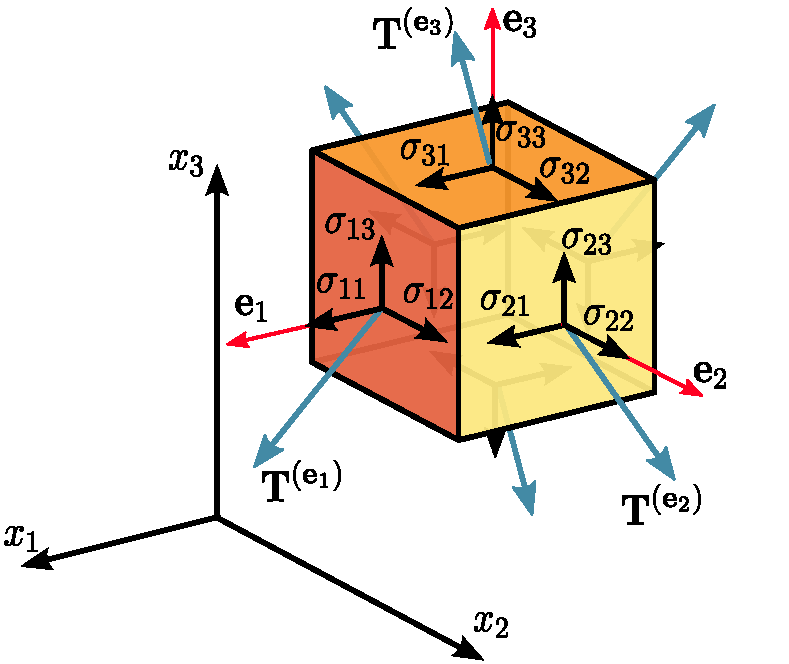
\includegraphics[width=0.8\textwidth]{figs/Components_stress_tensor_cartesian.pdf}
    \caption{Stress tensor wikipedia}\label{fig:stressTensor}
\end{figure}

%\begin{figure}[ht!]
%    \centering
%    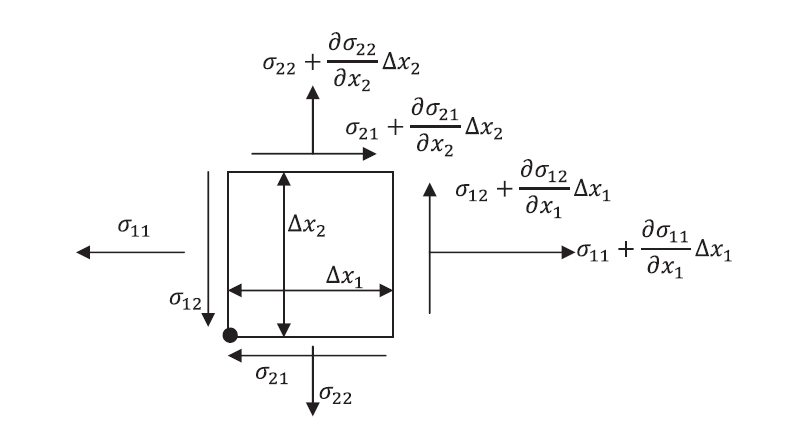
\includegraphics[width=0.8\textwidth]{figs/StressTensor.png}
%    \caption{Stress tensor 2D}
%\end{figure}

%\paragraph{Macro-Micro realtion} 
From a microscopic scale, the stress tensor describes the instantaneous local force from atomic interactions and momentum flux.
As a consequence of the scale, the tensor fluctuates strongly due to thermal motion, position and local arrangement of atoms.
The bridge between the microscopic description and the macroscopic scale is a spactial and statistical averaging of the microscopic stress over a region much larger than atomic dimensions\footnote{\[\sigma_{ij}^{\mathrm{macro}}=\lim_{V\to\infty}\expval{\sigma_{ij}^{\mathrm{micro}}}\]}.

%\subsection{Bridge of macro to micro stress tensor}

%\paragraph{Molecular stress is equivalent to continuum stress} 
%After exploring the constitutive equations and the main mechanisms related to the main mechanical responses observed in hydrogels, 
% 
This bridge it is no trivial, so we will demonstrate the validity of the connection between the macroscopic definition of the stress tensor with the microscopic stress tensor, by showing the equivalence between both tensors.
This mathematical derivation is adressed in the appendix of~\citep{admalUnifiedInterpretationStress2010}.
Just befor starting and for clarity, the notation is as follows,$\bm{\sigma}$ denotes a tensor, such as $\sigma_{i,j}$, a vector is denoted by $\vec{\sigma}$ and time average is denoted as $\overline{\sigma}$.

%\paragraph{Derivation} 
Let's start by considering a system of $N$ interacting particles with each particle position given by
\begin{equation}
    \vec{r}_{\alpha} = \vec{r} + \vec{s}_{\alpha}\label{eqn:DerVirTen1},
\end{equation}
where $\vec{r}$ is the position of the center of mass of the system and $\vec{s}_\alpha$ is the position of each point relative to the center of mass.
Hence, we can express the momentum of each particle as
\begin{equation}
    \vec{p}_\alpha = m_\alpha\qty(\dot{\vec{r}}+\dot{\vec{s}}_\alpha) = m_\alpha\qty(\dot{\vec{r}}+\vec{\upsilon}_\alpha^{\mathrm{rel}}).\label{eqn:DerVirTen2}
\end{equation}
Now lets recall that the center of mass of the system is given by
\begin{equation}
    \vec{r} = \frac{\sum_{\alpha}m_\alpha\vec{s}_\alpha}{\sum_{\alpha}m_\alpha}\label{eqn:DerVirTen3},
\end{equation}
and by replacing~\eqref{eqn:DerVirTen1} in~\eqref{eqn:DerVirTen2} we get the following relations, which will be used later,
\begin{equation}
    \sum_\alpha m_\alpha\vec{r}_\alpha = \vec{0},\quad
    \sum_\alpha m_\alpha\vec{\upsilon}_\alpha^{\mathrm{rel}} = \vec{0}.\label{eqn:DerVirTen4}
\end{equation}

Now we continue by computing the time derivative of tensorial product $\vec{r}_\alpha\otimes\vec{p}_\alpha$\footnote{It is interesting to note that the tensorial product $\vec{r}_\alpha\otimes\vec{p}_\alpha$ has units of action and by tacking the time derivative we are dealing with terms that has units of energy.
},
\begin{equation}
    \dv{t}\qty(\vec{r}_\alpha\otimes\vec{p}_\alpha) = 
    \underbrace{\vec{\upsilon}_\alpha^{\mathrm{rel}}\otimes\vec{p}_\alpha}_{\mathrm{Kinetic~term}} 
        +
        \underbrace{\vec{r}_\alpha\otimes\vec{f}_\alpha}_{\mathrm{Virial~term}},\label{eqn:DerVirTen5}
\end{equation}
which is known as the \textit{dynamical tensor virial theorem} and it is simply an alternative form to express the balance of linear momentum.
This theorem becomes useful after making the assumption that there existis a time scale $\tau$, which is short relative to macroscopic processes but long relative to the characteristic time of the particles in the system, over which the particles remain close to their original positions with bounded positions and velocities.
Taking advantage of this property we can compute the time average of~\eqref{eqn:DerVirTen5},
\begin{equation}
    \frac{1}{\tau}\qty(\vec{r}_\alpha\otimes\vec{p}_\alpha)\bigg|_{0}^{\tau} = 
    \overline{\vec{\upsilon}_\alpha^{\mathrm{rel}}\otimes\vec{p}_\alpha} 
        +
    \overline{\vec{r}_\alpha\otimes\vec{f}_\alpha}.\label{eqn:DerVirTen6}
\end{equation}
Assuming that $\vec{r}_\alpha\otimes\vec{p}_\alpha$ is bounded, and the time scales between microscopic and continuum processes are large enough, the term on the left-hand side can be as small as desired by tacking $\tau$ sufficiently large and by summing over all particles we achieve the \textit{tensor virial theorem}:
\begin{equation}
    \overline{\mathbf{W}} = -2\overline{\mathbf{T}},\label{eqn:DerVirTen7}
\end{equation}
where
\begin{equation}
    \overline{\mathbf{W}} = \sum_\alpha\overline{\vec{r}_\alpha\otimes\vec{f}_\alpha}\label{eqn:DerVirTen8}
\end{equation}
is the time-average virial tensor and
\begin{equation}
    \overline{\mathbf{T}}=\frac{1}{2}\sum_\alpha\overline{\vec{\upsilon}_\alpha^{\mathrm{rel}}\otimes\vec{p}_\alpha}\label{eqn:DerVirTen9}
\end{equation}
is the time-average kinetic tensor.
This expression for the tensor virial theorem applies equally to continuum systems that are not in macroscopic equilibrium as well as those that are at rest.

The assumption of the difference between the time scales allow us to simplify the relation by replacing~\eqref{eqn:DerVirTen2} in~\eqref{eqn:DerVirTen9}, so that,
\begin{equation}
    \overline{\mathbf{T}}=
        \frac{1}{2}\sum_\alpha m_\alpha\overline{\vec{\upsilon}_\alpha^{\mathrm{rel}}\otimes\vec{v}_\alpha^{\mathrm{rel}}}
        +
        \frac{1}{2} \left[\overline{\sum_\alpha m_\alpha\vec{\upsilon}_\alpha^{\mathrm{rel}}}\right]\otimes\dot{\vec{r}}\label{eqn:DerVirTen10},
\end{equation}
which is not the simplification we expected, however, by the relations from~\eqref{eqn:DerVirTen4}, equation~\eqref{eqn:DerVirTen10} simplifies to%\footnote{No estoy muy seguro si incluir una discusión acerca del término cinético en la expresión del virial. Posiblemente un párrafo\dots posiblemente lo ponga en la interpretación del teorema.
%También, no se si ir metiendo interpretación durante la derivación o no, pero bueno.}
\begin{equation}
    \overline{\mathbf{T}}=
        \frac{1}{2}\sum_\alpha m_\alpha\overline{\vec{\upsilon}_\alpha^{\mathrm{rel}}\otimes\vec{\upsilon}_\alpha^{\mathrm{rel}}}\label{eqn:DerVirTen11}.
\end{equation}
On the other hand, instead of reducing the expression, we start to create the conection with the Cauchy stress tensor by distributing~\eqref{eqn:DerVirTen8} into an internal and external contributions,
\begin{equation}
    \overline{\mathbf{W}} = 
    \underbrace{\sum_\alpha\overline{\vec{r}_\alpha\otimes\vec{f}_\alpha^{\mathrm{int}}}}_{\overline{\mathbf{W}}_{\mathrm{int}}}
        +
        \underbrace{\sum_\alpha\overline{\vec{r}_\alpha\otimes\vec{f}_\alpha^{\mathrm{ext}}}}_{\overline{\mathbf{W}}_{\mathrm{ext}}}.\label{eqn:DerVirTen12}
\end{equation}
The time-average internal virial tensor takes into account the interaction between particle $\alpha$ with the other particles in the system, meanwhile, the time-average external virial tensor considers the interaction with atoms outside the system, via a traction vector $\vec{t}$ and external fields acting on the system represented by $\rho\vec{b}$, where $\rho$ is the mass density of it and $\vec{b}$ is the body force per unit mass applied by the external field.
Therefore we can express the following,
\begin{equation}
    \sum_\alpha\overline{\vec{r}_\alpha\otimes\vec{f}_\alpha^{\mathrm{ext}}}
    :=
    \int_{\delta\Omega}\vec{\xi}\otimes\vec{t}dA 
    +
    \int_{\Omega}\vec{\xi}\otimes\rho\vec{b}dV.\label{eqn:DerVirTen13}
\end{equation}
Where $\vec{\xi}$ is a position vector within the domain $\Omega$ occupied by the system of particles with a continuous closed surface $\delta\Omega$.
Assuming that $\Omega$ is large enough to express the external forces acting on it in the form of the continuum traction vector $\vec{t}$.

With this we can substitute the traction vector with $\vec{t}=\bm{\sigma}\vec{n}$, where $\bm{\sigma}$ represent the Cauchy stress tensor and applying the divergence theorem in~\eqref{eqn:DerVirTen13}, we have 
\begin{equation}
    \overline{\mathbf{W}}_{\mathrm{ext}}
     =\int_{\Omega}
        \left[
            \vec{\xi}\otimes\rho\vec{b}+\mathrm{div}_{\vec{\xi}}\qty(\vec{\xi}\otimes\bm{\sigma})
        \right]dV
        =
    \int_{\Omega}
        \left[
            \bm{\sigma}^{\mathrm{T}}
            +
            \vec{\xi}\otimes\qty(\mathrm{div}_{\vec{\xi}}\bm{\sigma}+\rho\vec{b})
        \right]dV\label{eqn:DerVirTen14}
\end{equation}
Since we assume that we are under equilibrium conditions, the term $\mathrm{div}_{\vec{\xi}}\bm{\sigma}+\rho\vec{b}$ is zero~\eqref{eqn:DerVirTen14} it simplifies to
\begin{equation}
    \overline{\mathbf{W}}_{\mathrm{ext}}
    =V\bm{\sigma}^{\mathrm{T}}\label{eqn:DerVirTen15}.
\end{equation}
By tacking into account that we integrate over the domain $\Omega$ we can say that we compute the spatial average of the Cauchy stress tensor,
\begin{equation}
    \bm{\sigma}_{\mathrm{av}} =\frac{1}{V}\int_\Omega\bm{\sigma}dV\label{eqn:DerVirTen16},
\end{equation}
in which $V$ is the volume of the domain $\Omega$.
Replacing~\eqref{eqn:DerVirTen15} into~\eqref{eqn:DerVirTen12}, the tensor virial theorem~\eqref{eqn:DerVirTen7} can be expressed as,
\begin{equation}
    \sum_\alpha\overline{\vec{r}_\alpha\otimes\vec{f}_\alpha^{\mathrm{int}}}
    +
    V\bm{\sigma}_{\mathrm{av}}^{\mathrm{T}}
    =
    -\sum_\alpha m_\alpha\overline{\vec{\upsilon}_\alpha^{\mathrm{rel}}\otimes\vec{\upsilon}_\alpha^{\mathrm{rel}}}.\label{eqn:DerVirTen17}
\end{equation}
Finally, solving for the Cauchy Stress tensor we get,
\begin{equation}
    \bm{\sigma}_{\mathrm{av}}
    =
    -\frac{1}{V}
    \left[
        \sum_\alpha\overline{\vec{f}_\alpha^{\mathrm{int}}\otimes\vec{r}_\alpha}
        +
        \sum_\alpha m_\alpha\overline{\vec{\upsilon}_\alpha^{\mathrm{rel}}\otimes\vec{\upsilon}_\alpha^{\mathrm{rel}}}
    \right],\label{eqn:DerVirTen18}
\end{equation}
an expression that describe the macroscopic stress tensor in terms of microscopic variables\footnote{It is important to acknowledge that several mathematical subtleties were not taken into consideration, however all the mathematical formality is adressed by Nikhil Chandra Admal and E. B. Tadmor in~\citep{admalUnifiedInterpretationStress2010}}.

To end the demostration it is important to show that~\eqref{eqn:DerVirTen18} is symmetric.
Therefore, we rewrite the internal force as the sum of forces between the particles,
\begin{equation}
    \vec{f}^{\mathrm{int}}_\alpha = \sum_{{\beta}_{\beta\neq\alpha}}\vec{f}_{\alpha\beta}\label{eqn:DerVirTen19},
\end{equation}
and substituting~\eqref{eqn:DerVirTen19} into~\eqref{eqn:DerVirTen18}, we have
\begin{equation}
    \bm{\sigma}_{\mathrm{av}}
    =
    -\frac{1}{V}
    \left[
        \sum_{{\alpha,\beta}_{\beta\neq\alpha}}\overline{\vec{f}_{\alpha\beta}\otimes\vec{r}_\alpha}
        +
        \sum_\alpha m_\alpha\overline{\vec{\upsilon}_\alpha^{\mathrm{rel}}\otimes\vec{\upsilon}_\alpha^{\mathrm{rel}}}
    \right].\label{eqn:DerVirTen20}
\end{equation}
Due to the property $\vec{f}_{\alpha\beta}=-\vec{f}_{\beta\alpha}$ we obtain the following identity
\begin{equation}
    \sum_{{\alpha,\beta}_{\beta\neq\alpha}}\vec{f}_{\alpha\beta}\otimes\vec{r}_\alpha 
    =
    \frac{1}{2}\sum_{{\alpha,\beta}_{\beta\neq\alpha}}\left(\vec{f}_{\alpha\beta}\otimes\vec{r}_\alpha+\vec{f}_{\beta\alpha}\otimes\vec{r}_\beta\right)
    =
    \frac{1}{2}\sum_{{\alpha,\beta}_{\beta\neq\alpha}}\vec{f}_{\alpha\beta}\otimes\left(\vec{r}_\alpha-\vec{r}_\beta\right).\label{eqn:DerVirTen21}
\end{equation}
Therefore, by replacing the identity of~\eqref{eqn:DerVirTen21} into~\eqref{eqn:DerVirTen20}, we have
\begin{equation}
    \bm{\sigma}_{\mathrm{av}}
    =
    -\frac{1}{V}
    \left[
        \frac{1}{2}
        \sum_{{\alpha,\beta}_{\beta\neq\alpha}}\overline{\vec{f}_{\alpha\beta}\otimes\left(\vec{r}_\alpha-\vec{r}_\beta\right)}
        +
        \sum_\alpha m_\alpha\overline{\vec{\upsilon}_\alpha^{\mathrm{rel}}\otimes\vec{\upsilon}_\alpha^{\mathrm{rel}}}
    \right],\label{eqn:DerVirTen22}
\end{equation}
expressed with indexical notation and using the eistein summation convention,
\begin{equation}
    \sigma^{\mathrm{av}}_{ij}
    =
    -\frac{1}{V}
    \left[
        \frac{1}{2}
        \sum_{{\alpha,\beta}_{\beta\neq\alpha}}\overline{f^{\alpha\beta}_{i}r^\alpha_{j} + f^{\beta\alpha}_{i}r^\beta_{j}}
        +
        \sum_\alpha m_\alpha\overline{\upsilon^{\alpha~\mathrm{rel}}_{i}\upsilon^{\alpha{\mathrm{rel}}}_j}
    \right].\label{eqn:DerVirTen23}
\end{equation}
This allows us to quantify the relationship between the microscopic phenomena of a material with the macroscopic Cauchy stress tensor. 
Now, let's describe in general terms the relation between the elastic, plastic, viscoelastic and viscoplastic reponses with the microscopic phenomena.

%which is the same expression implemented in~LAMMPS\citep{LAMMPS}.\footnote{No se si poner la referencia a la pagina de documentacion}%\href{https://docs.lammps.org/compute_stress_atom.html}{https://docs.lammps.org/compute\_stress\_atom.html}}
%As a result, we can begin to explore which molecular process dominates each deformation regime.

%\paragraph{Elastic regime} 
In the case of an elastic deformation, the force applied to the material is largely retained.
This is due to the stretching of the distance between the particles.
The particles' displacement is minimal, with no effect on bond integrity.
This is generally understood to mean that the material stores potential energy that is released during unloading.

%\paragraph{Plastic regime}\footnote{Here it is important the idea of reversibility and stuf about self healing} 
In the context of plastic deformation, the phenomenon is often described as dislocation and crystal defects in crystalline materials.
However, given that the material under consideration is a polymeric network, plastic deformation is more likely to involve the rupture of crosslinks between chains and the sliding or stretching of individual chains beyond their reversible limit.
In the scenario of networks with physical entanglements, chains have the potential to slip past another, thereby overcoming energy barriers and irreversibly reorganizing the networks' topology.
In the cases of bond rupture, the crosslink density can be reduced or the polymeric chain can be broken.

%\paragraph{Viscoelastic regime} 
For this type of mechanical response, the network undergoes an elastic deformation.
However, during the elastic deformation process, the network may undergo changes in configuration due to polymer sliding or crosslinking reconfiguration.
During these changes, the interaction between polymer chains causes an energy dissipation process, resulting in a viscous response and a time dependency.
This time dependency is commonly known as \textit{stress relaxation}, which refers to the time-dependent decrease in stress under a constant, maintained strain.

%\paragraph{Viscoplastic regime} 
The viscoplastic response is comparable to the viscoelastic response because it integrates plastic deformation with an energy dissipation process.
The most significant distinction is that, in contrast to the elastic process of network sliding or crosslink reconfiguration, the polymeric network undergoes bond breakage.
Additionally, the disentanglement of chains is a significant phenomenon that plays a crucial role in energy dissipation.
Furthermore, the response is contingent on the time scale. 
The reconfiguration of the network is determined by the relaxation time following bond breakage and crosslinking reconfiguration.
Finally, similar to the plastic deformation, the viscoplastic deformation occurs after a yielding point, in which the deformation of the network structure is permanent.

\subsection{Hydrogel's mechanical response}

%\citep{bouzidElasticallyDrivenIntermittent2017}.

\paragraph{Intro}
In this section it is going to be a brief literature review from the reported mechanical response of hydrogel with the focus in searching for a connection between the strctural properties on a molecular level and the mechanical properties of the macroscopic hydrogel.
Lets start with the review article\citep{petelinsekToughHydrogelsLoadBearing2024}, in which they interpret the physical crosslinking mechansism as energy dissipation mechanisms.
This energy dissipation mechanisms helps to reversibly recover from a mechanical impact, allowing to create stiff and tough hydrogels.
The energy dissipation is often achieve through the introduction of sacrificial bonds by adding a second more brittle network within a loosly crosslinked network or by cross-links made from supramolecular transient interactions, which can be reversibly broken and reformed.
In the first case, the material is streched and a share of the bonds in the more brittle network are broken leading to an increased dissipation of the energy from mechanical impact.
In the second case, the sacrificial bonds are non-covalent nature and can reversibly break and reform.

Some of the non-covalent interactions are 
    metal–ligand, 
    ionic interactions, 
    hydrogen bonding, 
    microphase separation 
    and hydrophobic interactions, 
    polymer–nanomaterial adsorption, 
    host–guest complexation, 
    or supramolecular self-assembly.
However, in the review they center into the electrostatoc interaction, microphase separation, composites and self-assembly.
In figure~\ref{fig:energyDissipation} is a visual summary of the mechanisms that are going to be described in the following paragraphs.

From the electrostatic mechanism it can be said that ionic attractions between oppositly charged monomers led to tough, mechanically robust materials.
In addition, hydrogen bonds can be a powerful motif to enchance reversible interactions between polymer chains and hence, dissipate energy.

From the microphase sparation, it is important to acknowledge that microcrystallization is the process of polymer chains forming submicrometer-sized crystallites, representing a microphaseseparated domain surrounded by amorphous polymer chains.
Overall, hydrogels obtained through microcrystallization managed to improve the fracture energies and stiffness due to the collective hydrophobic interactions. 

From the composite mechanism it can be said that adding micellar agregates, soft polymers microspheres improve the thoughness of the hydrogel.
In addition, (nano)fibers may greatly enhance the fracture mechanics of tough hydrogels, however, their ductility often suffers greatly, especially when macroscopic fiber mats are inserted.

Finally, from the self-assembly mechanism, it can be said that is a promising source of energy dissipation have been introduced by elastomeric proteins, which function as molecular springs and unfold once a stress is applied. 
This mechanical unfolding can be observed in smaller elastin-like polypeptides, as well as in larger proteins

\begin{figure}[ht!]
    \centering
    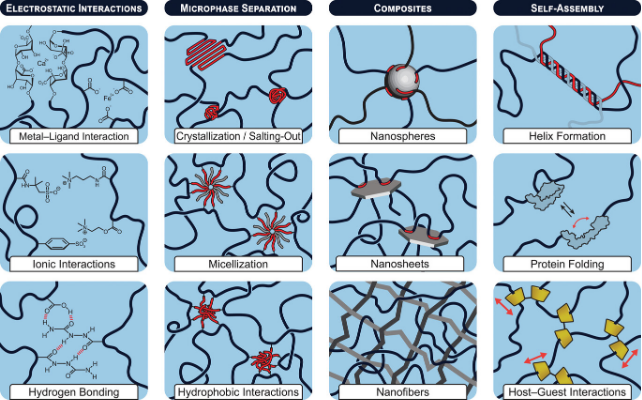
\includegraphics[width=0.7\textwidth]{figs/explainMechResponse/energyDissipationMechanisms.png
}
    \caption{Energy dissipation mechanism\citep{naritaViscoelasticPropertiesPolyvinyl2013}.}\label{fig:energyDissipation}
\end{figure}


\paragraph{Stress relaxation of a dual network}
The stress relaxation can be explain by the dynamics of association and dissasociation of chains\citep{naritaViscoelasticPropertiesPolyvinyl2013}.
In figure~\ref{fig:hydroMechResponse1} it is a comparison of a network with physical crosslinking mechanisms (left column) and a network with physical and chemical crosslink mechanisms (right row).
Taking a lot of attation into the physical elastically active and the physical elastically inactive positions, we can see the main difference is the functionality of the crosslinking.
The elastically active have a functionality greater than 2, meanwhile, the elastically inactive crosslinking has a functionality of 2. 

\begin{figure}[ht!]
    \centering
    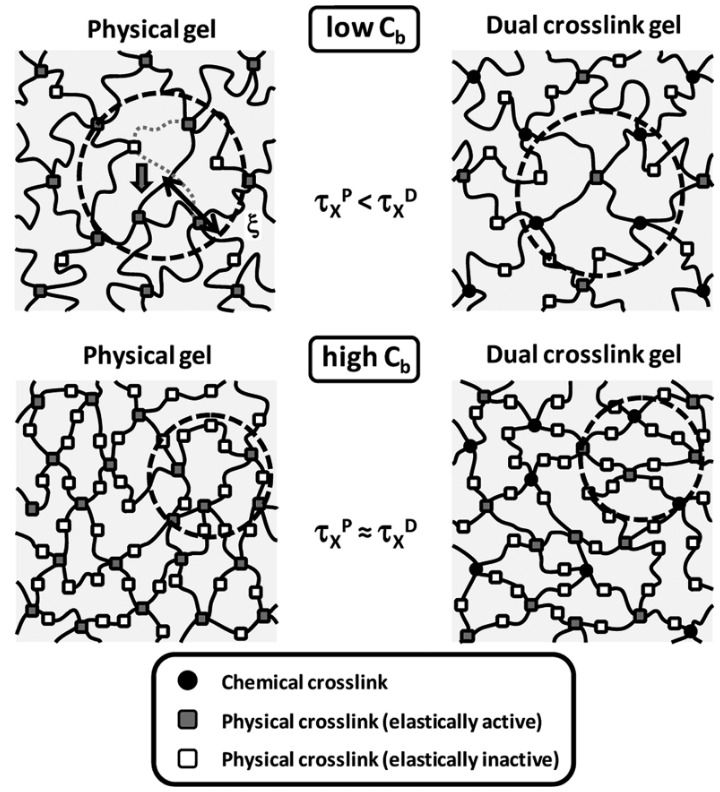
\includegraphics[width=0.7\textwidth]{figs/explainMechResponse/dualNetwork1.png}
    \caption{Stress relaxation mechanism for dual cross-linking mechanisms network\citep{naritaViscoelasticPropertiesPolyvinyl2013}.}\label{fig:hydroMechResponse1}
\end{figure}

When a chain is dissociated, this chain can be associated with any other elastically inactive crosslink within a distance.
This distance it is represented in the figure~\ref{fig:hydroMechResponse1} with a dashed circle.
And when the physical cross-linkers concentration is increase, two effects takes place.
One, the elastically active physical cross-link increases, decresing the time of association.
Second, increase the elastically inactive cross-links, which increases the time of association.
In this hydrogel the ''competition'' of this two effects results in the increase in the time of association, which induces an incomplete relaxation or the chain reassociates before complre stress relaxation.

\paragraph{Strain stifeening in dual networks}
In this other article\citep{kongEffectCrossLinkHomogeneity2024}, they prepare randomly cross-linked networks of poly(n-butyl acrylate) via thermally initiated free-radical polymerization and regularly cross-linked networks via thiol-bromine coupling of tetrafunctional poly(n-butyl acrylate) star polymers. 
Then they swell both types of networks in a mixture of monomer and cross-linker, which is polymerized to form double networks.
In order to explore the effect of cross-link homogeneity in the strain stiffening behavior of regular and random networks.

\begin{figure}[ht!]
    \centering
    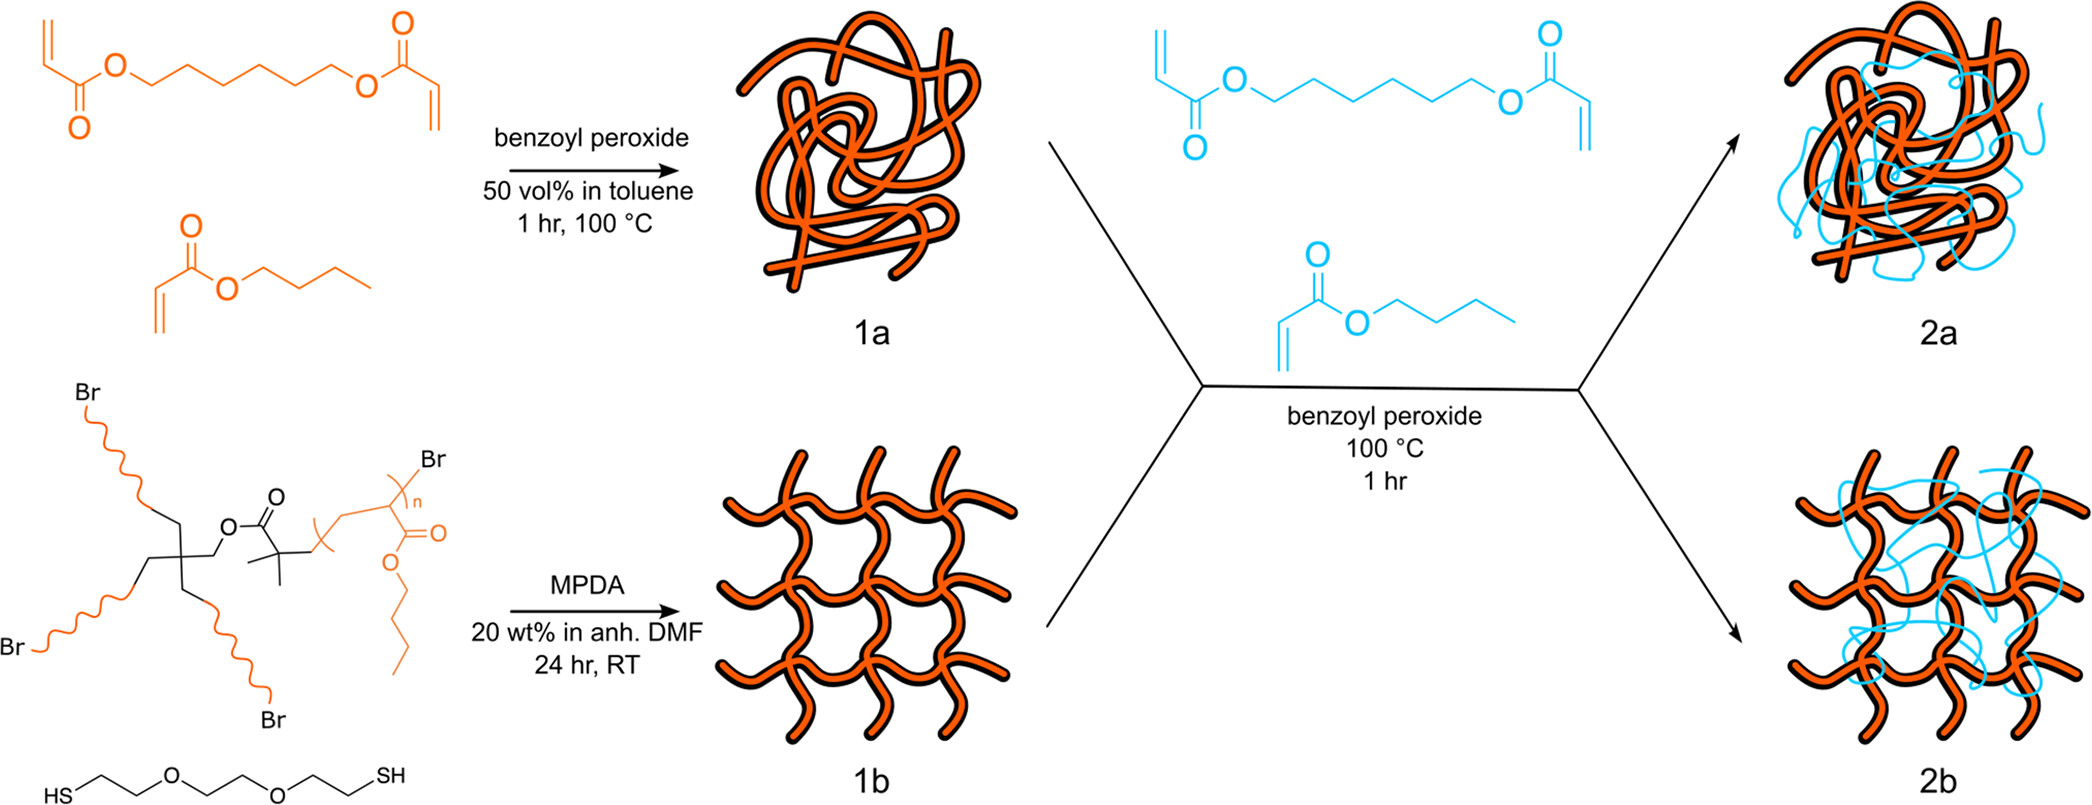
\includegraphics[width=0.75\textwidth]{figs/explainMechResponse/RAN-REG-networks.jpeg}
    \caption{Hydrogel's network configuration.
        Single network corresponds to 1a and 1b. 
        Double network corresponds to 2a and 2b.\citep{kongEffectCrossLinkHomogeneity2024}.}\label{fig:RANREGnetworks}
\end{figure}

In general terms, randomly cross-linked networks contain a polydisperse distribution of strand lengths with a high fraction of short strands and thus should strain harden at relatively low extensions. 
Meanwhile, regular networks, contain a much narrower distribution of predominantly higher molecular weight strands and should exhibit significantly delayed strain stiffening relative to comparable random networks.

First, in figure~\ref{fig:RANnetworks} are shown the strain-stress response of a single random hydrogel network with different crosslink concentration.
In the mechanical response, we can identify three distinct regimes: a linear elastic regime at low strain, a plateau at intermediate strain, and then a sharp increase in force at high strain, as the samples undergo strain stiffening.
It is important to notice that the strain at break increases when the crosslink concentration increases.
Also, the intermediate regime increases significantly with the concentration.

\begin{figure}[ht!]
    \centering
    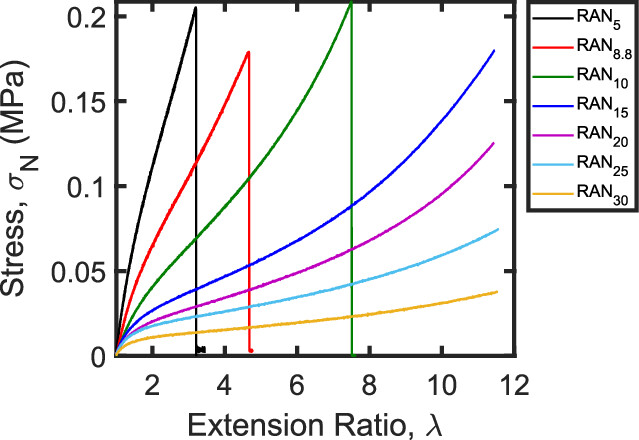
\includegraphics[width=0.75\textwidth]{figs/explainMechResponse/singleRANtensile.jpeg}
    \caption{Tensile response of random crosslink spatial distribution\citep{kongEffectCrossLinkHomogeneity2024}.}\label{fig:RANnetworks}
\end{figure}

Then, in figure~\ref{fig:RANnetworks} it is shown the mechanical response of a single regular hydrogel network with different crosslink concentration.
As before, when the crosslinker concentration increases the strain at breake increases.
On the other hand, in this type of hydrogel the plateau regime is lacking.

\begin{figure}[ht!]
    \centering
    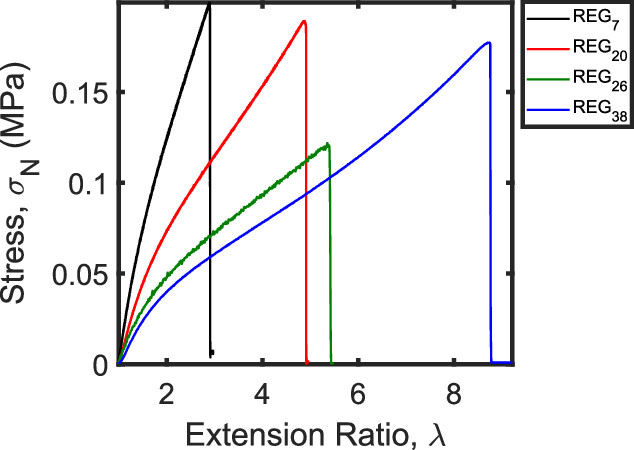
\includegraphics[width=0.75\textwidth]{figs/explainMechResponse/singleREGtensile.jpeg}
    \caption{Tensile response of regular crosslink spatial distribution\citep{kongEffectCrossLinkHomogeneity2024}.}\label{fig:REGnetworks}
\end{figure}

It is intereseting to notice that with a random network type the strain at break is higher than the strain at break of the regular network.
Furthermore, by looking at the same crosslinker concentration ($\mathrm{RAN}_{20}$ and $\mathrm{REG}_{20}$ )in both types of networks, the elastic response is more dominant in the regular network, meanwhile, the strain-stiffeing behaviour is more notisible in the random network. 

Once they characterize the single networks, they analyze the mechanical response onder tensile deformation of double network hydrogels.
In figure~\ref{fig:RANnetworks} we can see that the strain at break for the regular networks increases, while the strain at break of random network decreses. 
Also, in both types of networks we can see with more clarity the plastic, plateau and stiffeing regime.
Furthermore, the stiffening is enhance.
However, the plateau regime in the random networks shortens and the stiffening it is enhanced.
In contrast, in the regular network the plateau regime appears.
Finally, all of this is resume in the figure~\ref{fig:REGRANDNcomparison}. 

\begin{figure}[ht!]
    \centering
    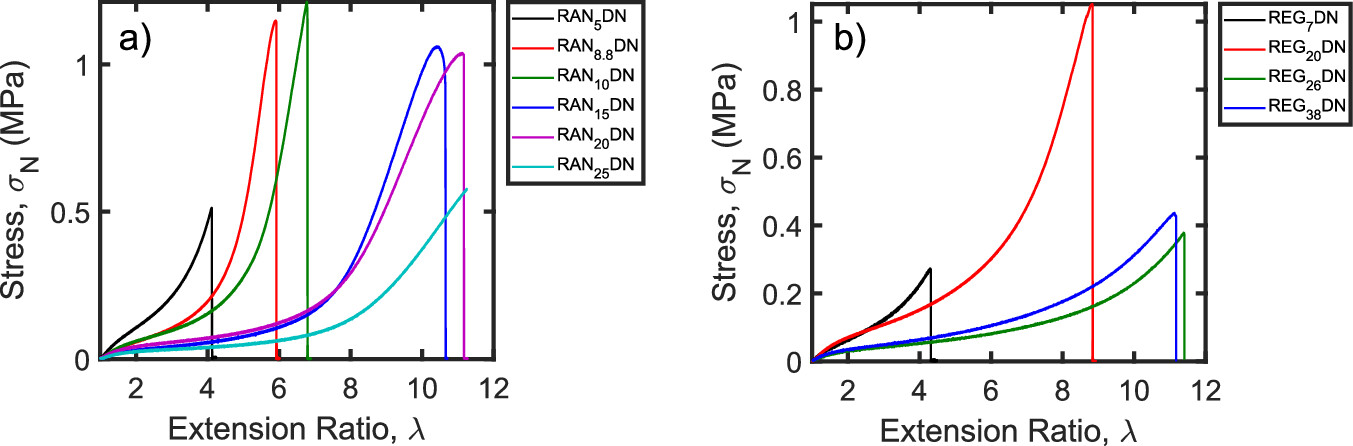
\includegraphics[width=0.75\textwidth]{figs/explainMechResponse/REGRANDN.jpeg}
    \caption{Tensile response of regular crosslink spatial distribution\citep{kongEffectCrossLinkHomogeneity2024}.}\label{fig:RANnetworks}
\end{figure}



\begin{figure}[ht!]
    \centering
    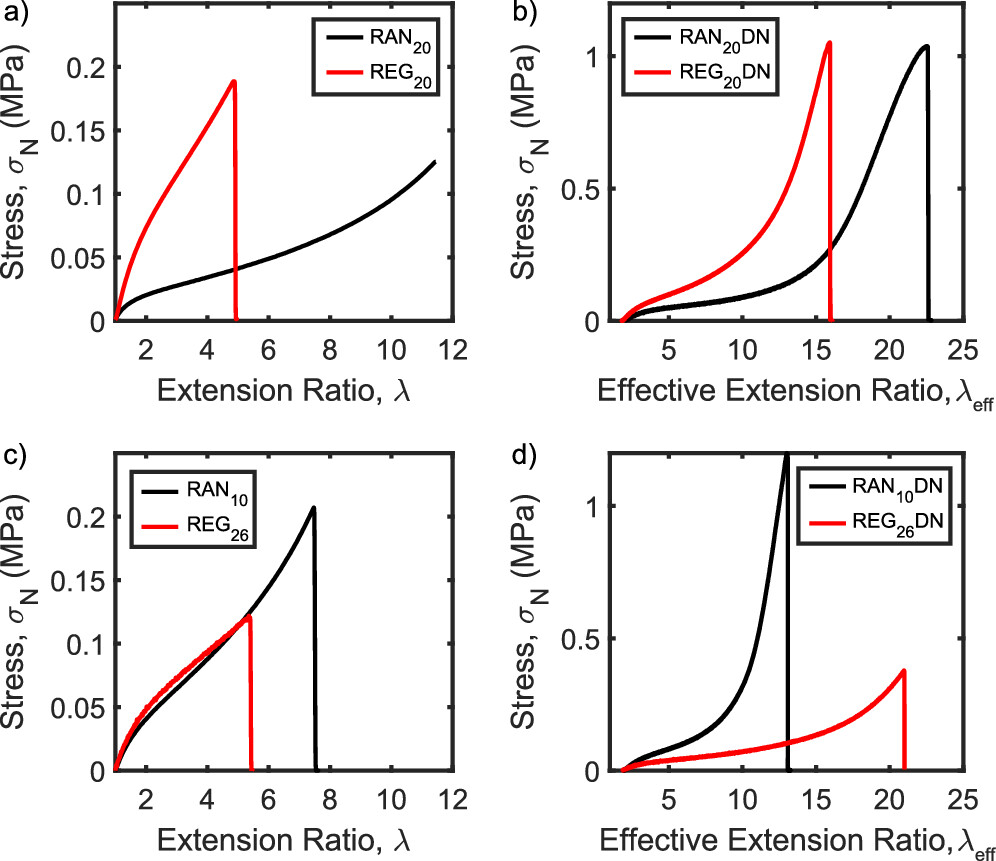
\includegraphics[width=0.75\textwidth]{figs/explainMechResponse/comparissonREGRANDN.jpeg}
    \caption{Tensile response of random crosslink spatial distribution\citep{kongEffectCrossLinkHomogeneity2024}.}\label{fig:REGRANDNcomparison}
\end{figure}


\paragraph{About shear thinning}
In the article\citep{varela-feijooMultiscaleInvestigationViscoelastic2023} analyze the viscoelastic properties of an alginate hydrogel.
For low concentrations the stifness and electrostatic repulsive interactions between chains and monomers are the main mechanisms that influence the viscosity.
However, when salt it is added to screen the electrostatic repulsions at the same low concentrations, the polymer chains contracted decreasin the volume occupied by a dosium alginate coil, causing a reduction in viscosity.
Then, by increasing the concentration of alginate, polymer chains become closer to the other leading to a solution in the semi-dilute entangled regime and a increase in viscosity.
Finally, when the hydrogel is above the concentrated regime, the electrostatic repulsion between chains become negligible and the density of entanglements increases, cause a further increment in the viscosity.
They report that this hydrogel also present shear-thinning as shown in figure~\ref{fig:hydroMechResponse2}.
That is when the shear rate it is increase, the shear viscosity decreases.
This behaviour can be explained by the disintanglement and alignment of alginate chains in the direction of the applied shear rate.

\begin{figure}[ht!]
    \centering
    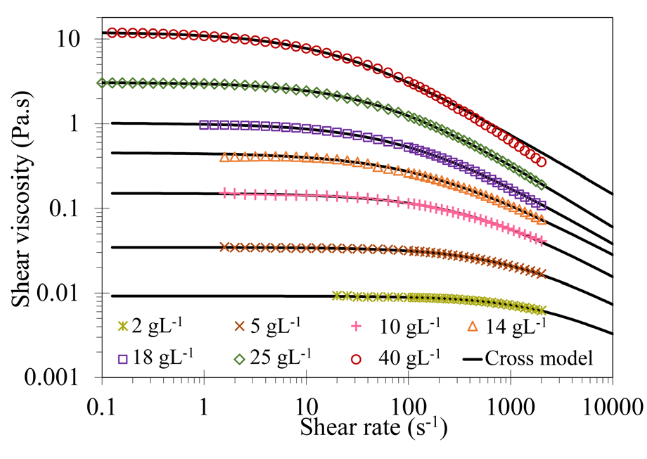
\includegraphics[width=0.75\textwidth]{figs/explainMechResponse/alginateShearThinning.png}
    \caption{Shear-thinning\citep{varela-feijooMultiscaleInvestigationViscoelastic2023}.}\label{fig:hydroMechResponse2}
\end{figure}






\begin{figure}[ht!]
    \centering
    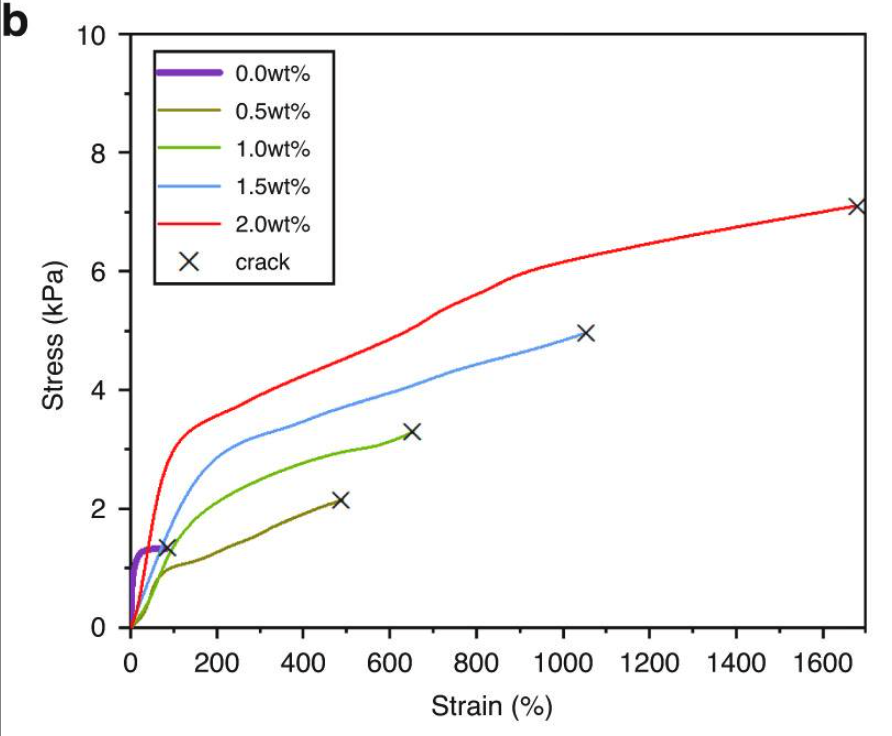
\includegraphics[width=0.7\textwidth]{figs/mechResponse/mech_response1.png}
    \caption{Tensile experiments. Strain-stress curve  of a novel bone-inspired fatigue-resistant hydrogel with excellent mechanical and piezoresistive properties from\citep{lyuBoneinspiredGNECHAPAAm2023}}
\end{figure}

\begin{comment}
\begin{figure}[ht!]
    \centering
    \begin{minifigure}[c]{with=0.5textwidth}
        \centering
        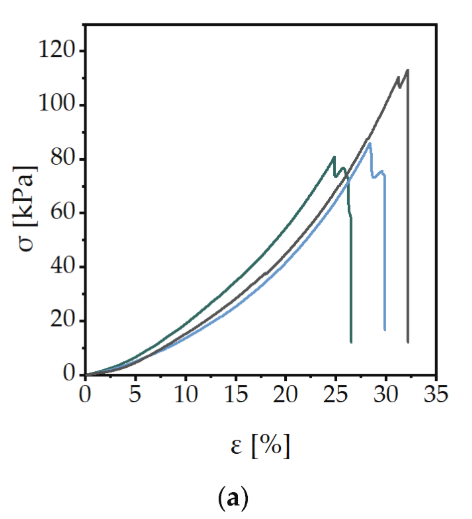
\includegraphics[width=\textwidth]{figs/mechResponse/2a.png}\caption{a}
    \end{minifigure}
    \begin{minifigure}[c]{with=0.5textwidth}
        \centering
        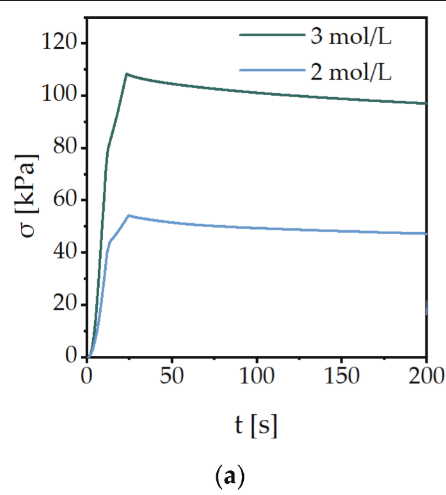
\includegraphics[width=\textwidth]{figs/mechResponse/2b.png}\caption{b}
    \end{minifigure}

    \begin{minifigure}[c]{with=0.5textwidth}
        \centering
        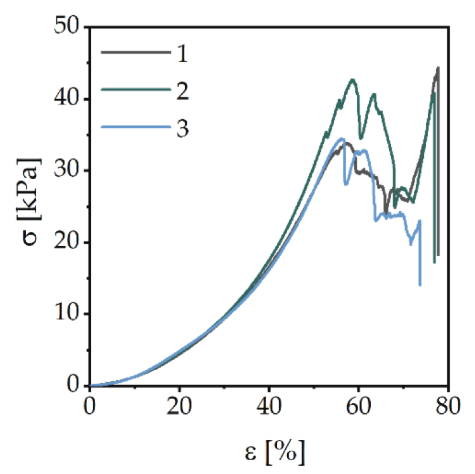
\includegraphics[width=\textwidth]{figs/mechResponse/2c.png}\caption{c}
    \end{minifigure}
    \caption{Tensile experiments\ref{romischkeSwellingMechanicalCharacterization2022}}
\end{figure}
\end{comment}

\begin{minipage}[c]{\textwidth}
\centering
\begin{minipage}[c]{0.45\textwidth}
    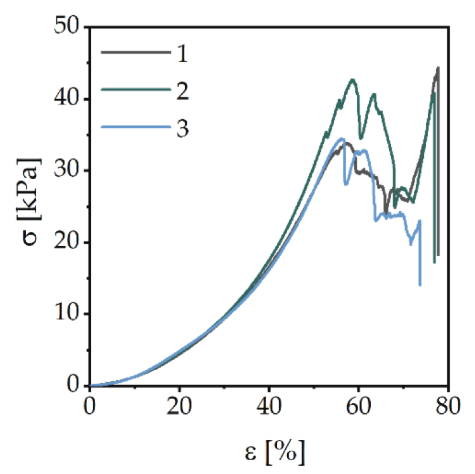
\includegraphics[width=\textwidth]{figs/mechResponse/2c.png}

    MASO3 (2 mol/L) with BAP (2 mol\%) as a crosslinker
\end{minipage}
\begin{minipage}[c]{0.45\textwidth}
    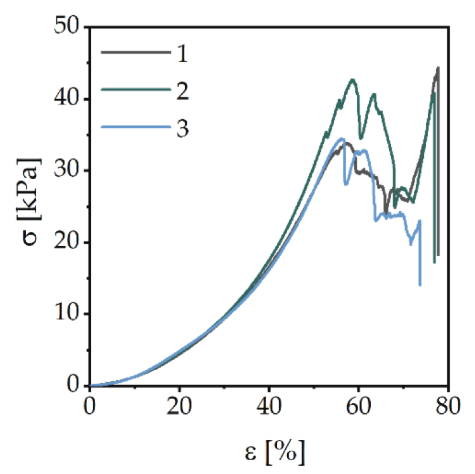
\includegraphics[width=\textwidth]{figs/mechResponse/2c.png}

     monomer AAMPSO3 (2 mol/L) with BAP (2 mol\%) as a crosslinker ($\epsilon$ = 8\%; n = 3)
\end{minipage}

\begin{minipage}[c]{0.45\textwidth}
    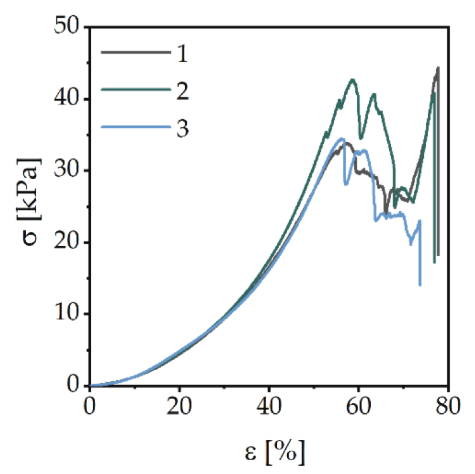
\includegraphics[width=\textwidth]{figs/mechResponse/2c.png}

    ChondroFiller liquid
\end{minipage}

Tensile experiments\ref{romischkeSwellingMechanicalCharacterization2022}

\end{minipage}

\begin{figure}[ht!]
    \centering
    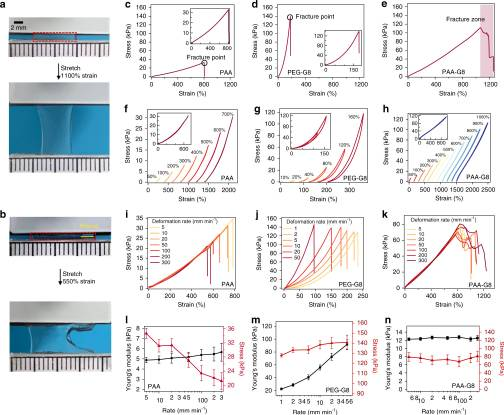
\includegraphics[width=0.7\textwidth]{figs/mechResponse/3.jpeg}
    \caption{Tensile tests from\citep{leiStretchableHydrogelsLow2020a}}
\end{figure}

\begin{figure}[ht!]
    \centering
    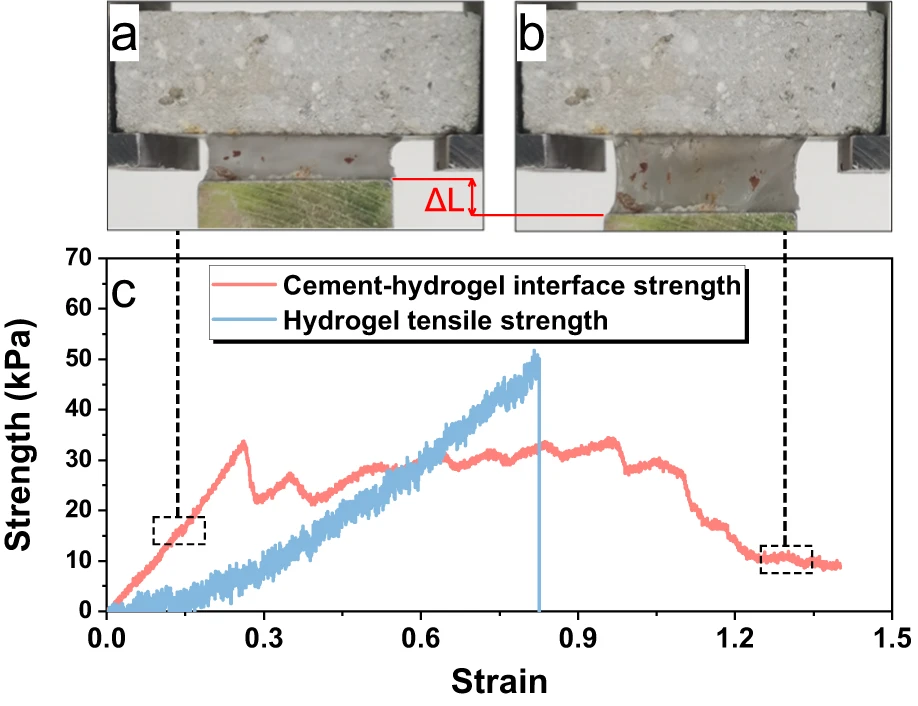
\includegraphics[width=0.7\textwidth]{figs/mechResponse/4.png}
    \caption{Tensile tests from\citep{chenMultilayeredCementhydrogelComposite2023}}
\end{figure}

\begin{figure}[ht!]
    \centering
    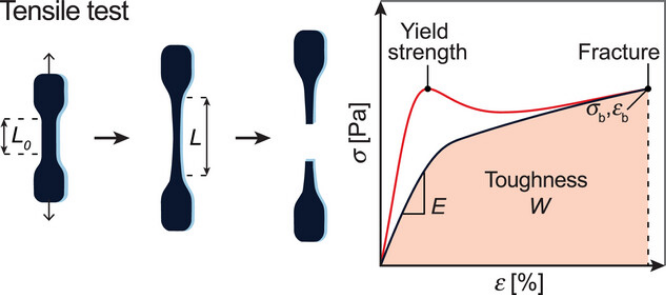
\includegraphics[width=0.7\textwidth]{figs/mechResponse/5.png}
    \caption{Tensile tests from\citep{petelinsekToughHydrogelsLoadBearing2024}. Uniaxial tensile test experiment of a plastically deforming material (red) and an elastic hydrogel (black).}
\end{figure}

\begin{figure}[ht!]
    \centering
    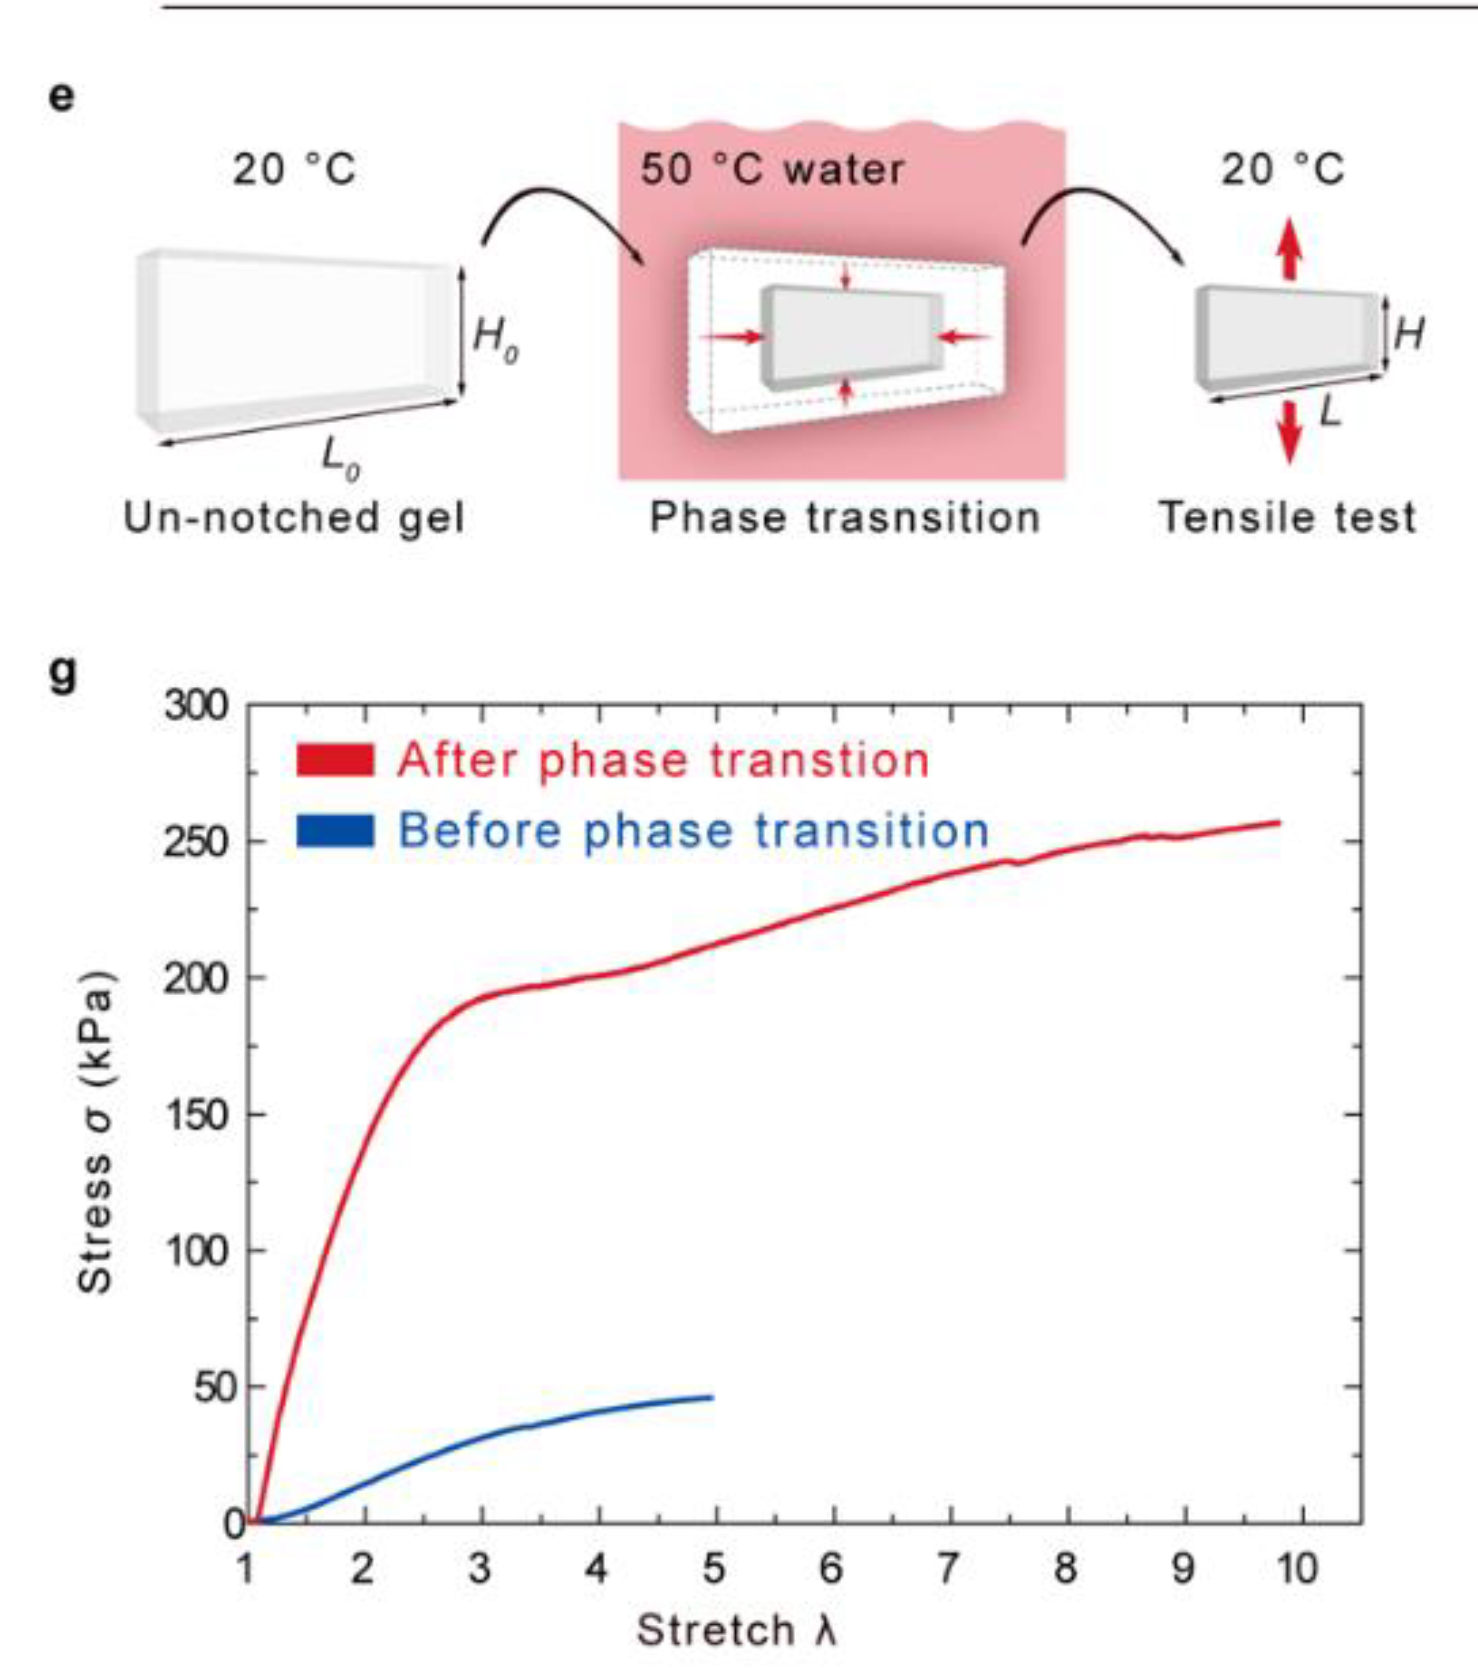
\includegraphics[width=0.7\textwidth]{figs/mechResponse/6.png}
    \caption{Tensile tests from\citep{kimFractureToughnessBlocking2022}}
\end{figure}

\begin{figure}[ht!]
    \centering
    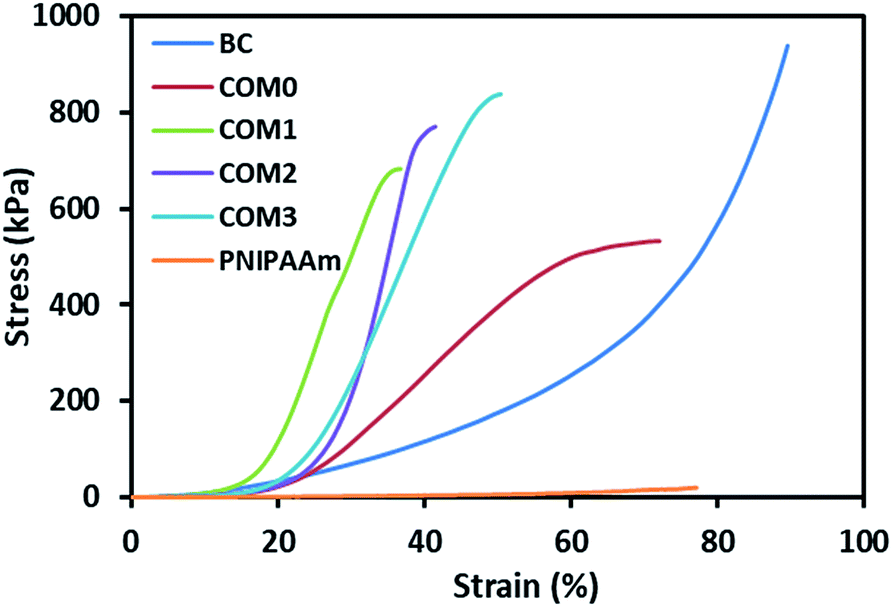
\includegraphics[width=0.7\textwidth]{figs/mechResponse/7.png}
    \caption{Compresive tests from\citep{wangRapidUniaxialActuation2018}}
\end{figure}

\begin{figure}[ht!]
    \centering
    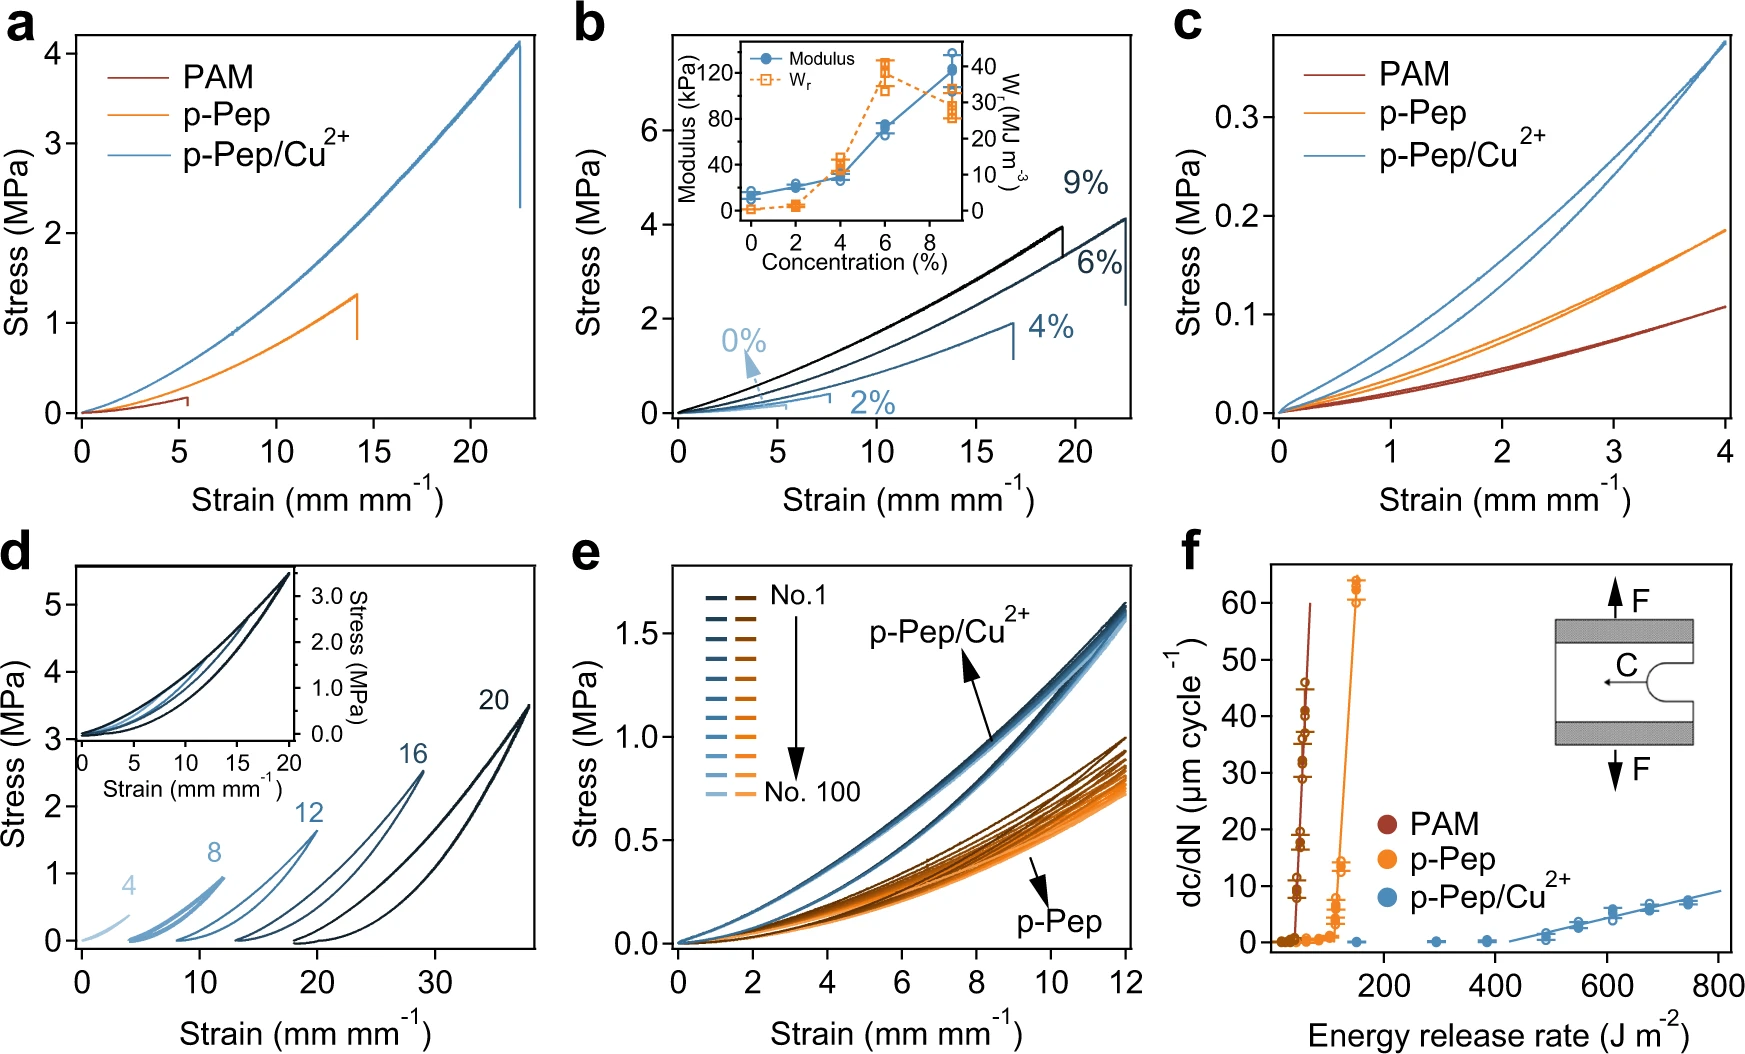
\includegraphics[width=0.7\textwidth]{figs/mechResponse/8.png}
    \caption{compresive tests from\citep{xuestrongtoughrapidrecovery2023}}
\end{figure}

\section{Molecular dynamics}

Now that we are familiarize with the mechanical response of the hydrogel and how the macroscopic and microscopic stress tensor are equivalent, in this section, we present the mathematical tools, also known as molecular dynamics (MD), employed to simulate the polymeric network.
Molecular dynamics is a widely used method for analyzing the mechanical responses of polymeric networks because it provides detailed insight into structure-property relationships.
This is due to its ability to represent atomic-level interactions via Newtonian mechanics, enabling the modeling of different crosslinking mechanisms, polymer chain configurations, time-dependent deformations, and others.
First, we will introduce the concept of colloids. 
Then, we will describe Langevin dynamics and explain how to solve them using the Velocity Verlet algorithm.

\subsection{Colloids}

We have explored the concepts of how a hydrogel can be understood as a polymeric network and how that helps to gain insight into the mechanical response and the different mechanical responses.
Now it is essential to introduce the concept of colloid to integrate the mathematical tools with the hydrogel representation as a polymeric network.

%\paragraph{Colloids} 
A colloid is a heterogeneous mixture of two substances in different matter states and in different ratio\citep{castaneda-priegoColloidalSoftMatter2021}.
It is commonly describe that one of the substance is dispersed into the other substance.
The disparsed substance it is commonly denoted as disparsed phase, while the other substance is denoted as the continuous phase.
The average size of the scattered phase's spots ranges from 1 nanometer to 1 micrometer.

This definition enables the classification of the material into the following eight categories:
foam, solid foam,
aerosol, emulsion, gel,
aerosol (solid), sol and solid sol.
As outlined in the table~\ref{tab:colloids}.
Naturally, our primary objective is to represent the hydrogel as a gel.

\begin{table}[ht!]
\begin{tabular}{|c|c|c|c|}
\hline
\textbf{Name of Colloid} & \textbf{Disparsed Phase} & \textbf{Continuous Phase} & \textbf{Examples}      \\ \hline
\textbf{Foam}            & Gas                      & Liquid                    & Whipped cream, froth   \\ \hline
\textbf{Solid Foam}      & Gas                      & Solid                     & Pumice, styrofoam      \\ \hline
\textbf{Aerosol}         & Liquid                   & Gas                       & Fog, mist              \\ \hline
\textbf{Emulsion}        & Liquid                   & Liquid                    & Milk, mayonnaise       \\ \hline
\textbf{Gel}             & Liquid                   & Solid                     & Jelly, cheese          \\ \hline
\textbf{Aerosol (solid)} & Solid                    & Gas                       & Smoke, airborne dust   \\ \hline
\textbf{Sol}             & Solid                    & Liquid                    & Paint, ink             \\ \hline
\textbf{Solid sol}       & Solid                    & Solid                     & Coloured glass, alloys \\ \hline
\end{tabular}
\caption{Types of colloids}\label{tab:colloids}
\end{table}

The hydrogel can be understood as a mixture of water in the liquid state and a polymer network in the solid state.
Furthermore, the polymeric network typically exhibits a porosity ranging from 5 to 20 nanometers, however they can be tunned to reach the micron-scale size.
This porosity enables the representation of the water as the dispersed phase, while the polymeric network is represented as the continuous phase.
Therefore, the hydrogel can be modelled as a colloidal gel.


\subsection{Langevin dynamics}

Now that we know that we can model a hydrogel as a colloid, we can start applying mathematical tools to create a quantitative description of the material.
Langevin dynamics is an excellent framework for representing this system, as it couples 
    the pairwise interactions of the polymers 
    with an efficient representation of the interaction of the water with the polymer, 
    and the dissipation of energy due that results from the water-polymer interaction.
It is important to note that this mathematical representation models an infinitesimal particle.
Therefore, a methodology is required that couples the infinitesimal particle with a polymer network.
The following methodology will be outlined following a description of the Langevin equation and the Velocity Verlet algorithm, in order to facilitate the process of storytelling.

%From a general point of view there are two types of methods to make a quatitative description of systems: one focused on simulating dynamics at the microscale, and the other dedicated to deriving or establishing evolutionary equations at the macroscale\citep{wangMultiscaleModelingSimulation2025}.
%At this scale there are two commonly used mathematical frameworks to model the molecular dynamics, the continuous time random walk (CTRW) model and the Langevin equation\citep{wangMultiscaleModelingSimulation2025}.

Taking into account the colloidal representation of the hydrogel, the Langevin theory takes advantage of the densities of the solid and liquid phases.
Since the solid phase of the colloid has a large mass, it will change their momenta after many collisions with the water molecules and the picture which emerges is that of the heavy particles forming a system with a much longer time scale than the solvent molecules\citep{Thijssen2007}.
This time scale difference can be used to our favour in the sense that we can eliminate the details of the degrees of freedom of the solvent particles and represent their effect by stochastic and dissipative forces allowing longer simulations that would be impossible if the solvent were explicitly included\citep{pastorTechniquesApplicationsLangevin1994}.

However, the representation of the solvent by a stochastic and dissipative force, introduce the problem of characterize two very different timescales.
One associated with the slow relaxation of the initial velocity of the particle and another linked to the frequent collisions that the particle suffers with particles of the bath\citep{tsl2006}. 
Therefore, two terms are used to create a mathematical representation of the solvent: a frictional force proportional to the velocity of the particle and a fluctuating force. 

By considering newtonian mechanics and the previous discussion, the Langevin dynamics are mathematically represented by the following differential equation,
\begin{gather}
    m\dv{\vec{v}(t)}{t}=\vec{F}(t)-\gamma\vec{v}(t)+\vec{R}(t).\label{eqn:BrownianDyn1}
\end{gather}
The term in the left-hand size of the equation denotes the change of momentum of the particle.
The first term on the right-hand side of the equation represents the force due to the interaction of the particle with other particles.
The second term couples the dissipation of energy of the particle due to its interaction with the solvent.
Finally, the third term takes into account the exchange of momenta with the solvent.

The friction constant $\gamma$ parametrises the effect of solvent damping and activation and has units \SI{}{\kilo\gram\per\second}.
It is commonly referred as the collision frequency in the simulation literature, even though formally a Langevin description implies that the solute suffers an infinite number of collisions with infinitesimally small momentum transfer.
Furthermore, the fact that the second term is not a function of the position of any of the particles involves the neglect of hydrodynamic interaction or spatial correlation in the friction kernel\citep{pastorTechniquesApplicationsLangevin1994}.

On the other hand, the term $\vec{R}(t)$ is a ``random force'' subject to the following conditions
\begin{gather}
    \expval{\vec{R}(t)} = 0\label{eqn:LagDynamicNoiseExpval} \\
    \expval{\vec{R}(t)\vec{R}(t')} = 2k_{B}T\gamma\delta\qty(t-t')\label{eqn:LagDynamicNoiseCorrelation} 
\end{gather}
The no time correlation is equivalent to assuming that the viscoelastic relaxation of the solvent is very rapid with respect to solute motions\citep{pastorTechniquesApplicationsLangevin1994}.
%\footnote{Grote land Hynes [26] have investigated this assumption for motions involving barrier crossing and have found that while it is seriously in error for passage over sharp barriers (such as 12 recombination); it is quite adequate for conformational transitions such as might be found in polymer motions.}

In comparing the results of Langevin dynamics with those of other stochastic methods, the relevant variable is the velocity relaxation time, $\tau_{v}$ which equals $\gamma^{-1}$\citep{pastorTechniquesApplicationsLangevin1994}
The Langevin equation improves conformational sampling over standard molecular dynamics\citep{paquetMolecularDynamicsMonte2015}.

%    \item hablar de la ecuación de Green-Kubo: \[\eta=\frac{V}{k_B T}\int_{0}^{\infty}\expval{\sigma_{xy}(t)\sigma_{xy}(0)}\mathrm{d}t\]

\subsection{Velocity Verlet}

%\paragraph{Intro}
In order to solve the Langevin equation~\eqref{eqn:BrownianDyn1} we apply the Velocity Verlet numerical method.
The core concept of the Velocity Verlet algorithm is to update particle positions and velocities using both current and predicted accelerations, ensuring time-reversibility and energy conservation over long simulations. 
From a mathematical point of view, this algorithm is a second-order integrator for ordinary differential equations and is based on truncated Taylor expansion.
Which for a particle with mas $m$, position $r(t)$, and force $f(r,t)$, the velocity Verlet schemes is express as
\begin{align}
    r^{n+1} &= r^n + v^n dt + \frac{dt^2}{2m}f^n \\
    v^{n+1} &= v^n + \frac{dt}{2m}(f^n+f^{n+1}).
\end{align}
Furthermore, from a computational perspective, Velocity Verlet is an explicit algorithm, easy to implement, and efficient in term of memory usage.
It requires only the positions, velocities, and accelerations from the previous timestep.
Which allows efficient parallelization and eliminates the need for additional memory allocations per step.

A modified version of this scheme is the Stormer-Verlet method. 
This involves considering two successive time steps and eliminating the velocity variables, leading to the following expression,
\begin{align}
    r^{n+1} + 2r^{n} - r^{n-1} + \frac{dt^2}{m}f^{n},
\end{align}
with the associated velocity calculated by the central difference
\begin{align}
    v^n = \frac{r^{n+1} - r^{n-1}}{2dt}.
\end{align}
This is important because the software used for the molecular dynamics implements this version of the velocity verlet.

In systems governed by Langevin dynamics, the algorithm can incorporate random forces consistent with the fluctuation-dissipation theorem to simulate physically realistic Brownian motion.
Howver, the non-analytical term $\vec{R}(t)$ from equation~\eqref{eqn:BrownianDyn1} invalidates the Taylor expansion used for the derivation of the Verlet scheme.
Hence, in order to develop a reliable integrator for Langevin dynamics one therefore needs to carefully treat the copupling between the stochastic and analytic contributions.
Therefore, we are going to show the derivation of the Stormer-velocity Verlet scheme for the Langevin equation following the process shown in \citep{gronbech-jensenSimpleEffectiveVerlettype2013a}.

The first step is to translate the continuous variable $t$ to a discrete variable.
In order to accomplish that, we integrate the equation\eqref{eqn:BrownianDyn1} over a small time interval $dt$ from $t_n$ to $t_{n+1}=t_{n}+dt$,
\begin{align}
    \int_{t_n}^{t_{n+1}}m\dv{\vec{v}(t)}{t}dt'
    =
    \int_{t_n}^{t_{n+1}}\vec{F}(t)dt'
    -\int_{t_n}^{t_{n+1}}\gamma\vec{v}(t)dt'
    +\int_{t_n}^{t_{n+1}}\vec{R}(t')dt',
\end{align}
which it is equal to
\begin{align}
    m\qty(\vec{v}^{n+1} - \vec{v}^{n})
    =
    \int_{t_n}^{t_{n+1}}\vec{F}(t)dt'
    -\gamma\qty(r^{n+1}-r^n)
    +\int_{t_n}^{t_{n+1}}\vec{R}(t')dt'\label{eqn:DerVelVerlet1}.
\end{align}

Now, recalling that,
\begin{gather}
    \dv{\vec{r}}{t} = v,
\end{gather}
we can integrate over a small time interval and get,
\begin{gather}
    \int_{t_n}^{t_{n+1}}\dv{\vec{r}}{t} dt' = \vec{r}^{n+1}-\vec{r}^{n} = \int_{t_n}^{t_{n+1}}\vec{v} dt'.
\end{gather}
The left hand side can be approximated with forward finite differences,
\begin{gather}
    \vec{r}^{n+1}-\vec{r}^{n} \approx \frac{dt}{2}\qty(\vec{v}^{n+1} + \vec{v}^n)\label{eqn:DerVelVerlet2}.
\end{gather}
Solving for $\vec{v}^{n+1}$ from equation~\eqref{eqn:DerVelVerlet1} we get the following expression for the velocity,
\begin{gather}
    \vec{v}^{n+1} = \frac{1}{m}\int_{t_n}^{t_{n+1}}\vec{F}(t)dt'
                     -\frac{\gamma}{m}\qty(r^{n+1}-r^n)
                     +\frac{1}{m}\int_{t_n}^{t_{n+1}}\vec{R}(t')dt'
                     +\vec{v}^{n}\label{eqn:DerVelVerlet3}.
\end{gather}
Replacing the term $\vec{v}^{n+1}$ in equation~\eqref{eqn:DerVelVerlet2} with equation~\eqref{eqn:DerVelVerlet3} and some algebraic manipulation we get,
\begin{equation}
    \vec{r}^{n+1} = \frac{m dt}{2m +\gamma dt}\left[ 
                        2\vec{v}^{n}                
                        +\frac{1}{m}\int_{t_n}^{t_{n+1}}\vec{F}(t)dt'
                        +\frac{1}{m}\int_{t_n}^{t_{n+1}}\vec{R}(t')dt'
                    \right]
                    +r^n\label{eqn:DerVelVerlet4}.
\end{equation}
Now we need are going to tackle the integral of force in equations~\eqref{eqn:DerVelVerlet3} and~\eqref{eqn:DerVelVerlet4}.
Since is a deterministic force, we can approximate the integral such that both equations are correct to second order in $dt$ and have the follwong pair of equations,
\begin{align}
    \vec{r}^{n+1} &= r^n
                    +\frac{m dt}{2m +\gamma dt}\left[ 
                        2\vec{v}^{n}                
                        +\frac{dt}{m}F^{n}
                        +\frac{1}{m}\int_{t_n}^{t_{n+1}}\vec{R}(t')dt'
                    \right]\label{eqn:DerVelVerlet5}
                    , \\
    \vec{v}^{n+1} &= \vec{v}^{n}
                     +\frac{1}{m}\frac{dt}{2}\qty(\vec{F}^{n} + \vec{F}^{n+1})
                     -\gamma\qty(r^{n+1}-r^n)
                     +\frac{1}{m}\int_{t_n}^{t_{n+1}}\vec{R}(t')dt'\label{eqn:DerVelVerlet6}.
\end{align}
Finally, the integral over the random force is going to give another random variable with the same conditions of equations~\eqref{eqn:LagDynamicNoiseExpval} and~\eqref{eqn:LagDynamicNoiseCorrelation}, hence we can define the following,
\begin{gather}
    \vec{\eta}^{n+1}\equiv\int_{t_n}^{t_{n+1}}\vec{R}(t')dt'\label{eqn:DerVelVerlet7},
\end{gather}
with $\expval{\eta^{n}}=0$ and $\expval{\eta^{n}\eta^{l}}=2k_{B}T\gamma\delta\qty(t-t')$.
Replacing~\eqref{eqn:DerVelVerlet7} into equations~\eqref{eqn:DerVelVerlet5} and~\eqref{eqn:DerVelVerlet6} we get the scheme to solve Langevin equation using the Velocity Verlet scheme,
\begin{align}
    \vec{r}^{n+1} &= r^n
                    +\frac{m dt}{2m +\gamma dt}\left[ 
                        2\vec{v}^{n}                
                        +\frac{dt}{m}F^{n}
                        +\frac{1}{m}\vec{\eta}^{n+1}
                    \right]\label{eqn:DerVelVerlet5}
                    , \\
    \vec{v}^{n+1} &= \vec{v}^{n}
                     +\frac{1}{m}\frac{dt}{2}\qty(\vec{F}^{n} + \vec{F}^{n+1})
                     -\gamma\qty(r^{n+1}-r^n)
                     +\frac{1}{m}\vec{\eta}^{n+1}\label{eqn:DerVelVerlet6}.
\end{align}
It is interesting to notice that the noise is represented as a single stochastic varaible for each time step, realized by a single agregated impulse during $dt$ that influences the dynamics over the time step.
Finally, it is important to notice that $\vec{F}^{n}$, $\vec{F}^{n+1}$ and $\vec{\eta}^{n+1}$ have units of momenta \SI{}{\kilo\gram\meter\per\second} and the constant $\frac{m dt}{2m +\gamma dt}$ has units of time \SI{}{\second}. 

\begin{comment}
\begin{gather}
    \vec{r}^{n+1} = \frac{dt}{2}\left[ 
                        \frac{1}{m}\int_{t_n}^{t_{n+1}}\vec{F}(t)dt'
                        -\frac{\gamma}{m}\qty(r^{n+1}-r^n)
                        +\frac{1}{m}\int_{t_n}^{t_{n+1}}\vec{R}(t')dt'
                        +2\vec{v}^{n}
                    \right]
                     +\vec{r}^n.
\end{gather}

\begin{equation}
    \vec{r}^{n+1} = -\frac{dt}{2}\frac{\gamma}{m}\qty(r^{n+1}-r^n)
                    +
                    \frac{dt}{2}\left[ 
                        \frac{1}{m}\int_{t_n}^{t_{n+1}}\vec{F}(t)dt'
                        +\frac{1}{m}\int_{t_n}^{t_{n+1}}\vec{R}(t')dt'
                        +2\vec{v}^{n}
                    \right]
                     +\vec{r}^n.
\end{equation}


\begin{equation}
    \vec{r}^{n+1} = -\frac{dt}{2}\frac{\gamma}{m} r^{n+1}+\frac{dt}{2}\gamma r^n
                    +
                    \frac{dt}{2}\left[ 
                        \frac{1}{m}\int_{t_n}^{t_{n+1}}\vec{F}(t)dt'
                        +\frac{1}{m}\int_{t_n}^{t_{n+1}}\vec{R}(t')dt'
                        +2\vec{v}^{n}
                    \right]
                     +\vec{r}^n.
\end{equation}

\begin{equation}
    \vec{r}^{n+1}\qty(1+\frac{dt}{2}\frac{\gamma}{m}) = \frac{dt}{2}\gamma r^n
                    +
                    \frac{dt}{2}\left[ 
                        \frac{1}{m}\int_{t_n}^{t_{n+1}}\vec{F}(t)dt'
                        +\frac{1}{m}\int_{t_n}^{t_{n+1}}\vec{R}(t')dt'
                        +2\vec{v}^{n}
                    \right]
                     +\vec{r}^n.
\end{equation}

\begin{equation}
    \vec{r}^{n+1}\qty(1+\frac{dt}{2}\frac{\gamma}{m}) = 
                    \frac{dt}{2}\left[ 
                        \frac{1}{m}\int_{t_n}^{t_{n+1}}\vec{F}(t)dt'
                        +\frac{1}{m}\int_{t_n}^{t_{n+1}}\vec{R}(t')dt'
                        +2\vec{v}^{n}
                    \right]
                     +\frac{dt}{2}\gamma r^n
                    +\vec{r}^n.
\end{equation}

\begin{equation}
    \vec{r}^{n+1}\qty(1+\frac{dt}{2}\frac{\gamma}{m}) = 
                    \frac{dt}{2}\left[ 
                        \frac{1}{m}\int_{t_n}^{t_{n+1}}\vec{F}(t)dt'
                        +\frac{1}{m}\int_{t_n}^{t_{n+1}}\vec{R}(t')dt'
                        +2\vec{v}^{n}
                    \right]
                     +r^n\qty(\frac{dt}{2}\gamma + 1)
                    .
\end{equation}

\begin{equation}
    \vec{r}^{n+1} = \frac{dt}{2\qty(1+\frac{dt}{2}\frac{\gamma}{m})}\left[ 
                        \frac{1}{m}\int_{t_n}^{t_{n+1}}\vec{F}(t)dt'
                        +\frac{1}{m}\int_{t_n}^{t_{n+1}}\vec{R}(t')dt'
                        +2\vec{v}^{n}
                    \right]
                    +\frac{\qty(\frac{dt}{2}\gamma + 1)}{\qty(1+\frac{dt}{2}\gamma)}r^n
                    .
\end{equation}

\begin{equation}
    \vec{r}^{n+1} = \frac{dt}{2+\gamma dt}\left[ 
                        \frac{1}{m}\int_{t_n}^{t_{n+1}}\vec{F}(t)dt'
                        +\frac{1}{m}\int_{t_n}^{t_{n+1}}\vec{R}(t')dt'
                        +2\vec{v}^{n}
                    \right]
                    +\frac{2+dt\gamma}{2+dt\gamma}r^n
                    .
\end{equation}

\end{comment}






\begin{comment}
    \vec{v}^{n+1}
    =
    \frac{1}{m}
    \int_{t_n}^{t_{n+1}}\vec{F}(t)dt'
    -\gamma\qty(r^{n+1}-r^n)
    +\frac{1}{m}\int_{t_n}^{t_{n+1}}\vec{R}(t')dt'
    +\vec{v}^{n}
\end{comment}

Since we need to solve the equation~\eqref{eqn:BrownianDyn1} for a $N$ particle system, the implementation of the Velocity Verlet scheme for a many-particle system is computationally handled by the LAMMPS molecular dynamics software.
A key benefit of this choice is that LAMMPS comes well-equipped with robust and scalable parallel computing schemes, enabling the efficient simulation of large systems. 
This pre-existing, optimized framework is crucial, as developing a parallelized numerical solver from the ground up would be prohibitively time-consuming and complex. 
This allows us to concentrate our efforts on designing the polymer network models and analysing their resulting mechanical properties, rather than on the simulation engine itself.

\subsection{LAMMPS}

LAMMPS (Large-scale Atomic/Molecular Massively Parallel Simulator) is a highly flexible, open-source molecular dynamics software solution used for simulating atomic, molecular, and mesoscale systems. 
And is widely recognized for its extensibility, complete documentation, and active support in scientific communities focused on materials modeling and molecular simulation.
It is designed to efficiently model materials science, chemistry, and physics problems by enabling large-scale simulations on parallel computing architectures.
Furthermore, its parallelized structure allows efficient computation of large or complex systems, and supports integration with other computational tools and machine learning methods.

To define a simulation with this software we need to create an input script.
This input script is defined as a series of lines, with each line beginning with a command name and followed by one or more arguments separated by whitespace.
The program incorporates programming commands that define variables, perform conditional tests, execute loops, or invoke shell commands to launch an external program.
The input script is parsed and executed one line at a time. 
This feature allows a single script to run a simulation in stages, alter one or more parameters between stages, or run a series of independent simulations where the entire system is reinitialized multiple times.

The Langevin equation in LAMMPS is implemented as follows,
\begin{align}
    F &= F_c -\frac{m}{\mathrm{damp}}v + F_r,\label{eqn:MolDylammps1} \\
    F_r &\propto\sqrt{\frac{k_B T m}{dt\mathrm{damp}}},\label{eqn:MolDylammps2}
\end{align}
where $F_c$ is the conservative force computed from particle-particle interactions.
The term $F_r$ is equivalent to $-m\gamma v$ and $F_r$ is equivalent to the term $\vec{R}(t)$ on equation~\eqref{eqn:BrownianDyn1}.
LAMMPS implements the random numbers to randomize the direction and magnitude of this force, where a uniform random number is used (instead of a Gaussian random number) for speed.

The magnitud of the random force is derived from the fluctuation/dissipation theorem, where $k_B$ is the Boltzmann constant, $T$ is the desired temperature, $m$ the mass of the particle, $dt$ the timestep size and $\mathrm{damp}$ is the damping factor.
The damp factor can be thought of as inversely related to the viscosity of the solvent.
That is a small relaxation time implies a high-viscosity solvent and vice versa.
This parameter is specified in time units and determines how rapidly the temperature is relaxed.

On the other hand, to use the velocity verlet scheme previously discussed, we need to used the command \verb|fix nve|.
Although the command makes allution to the NVE enssemble, what really does is to invoke the velocity form of the Stoermer-Verlet time integration algorithm (velocity-Verlet).
The combination of \verb|fix langevin| and \verb|fix nve| allow us to perform molecular dynamics with particle-particle interaction for a many particle system.

